\documentclass[a4paper, 12pt]{article}
\newcommand{\template}{../../Templates}
\usepackage{\template/package}
\graphicspath{{../../Assets/}}

\newcommand{\Titolo}{Analisi dei requisiti}
\newcommand{\Data}{17/11/2023}
\newcommand{\Versione}{0.1.0}
\newcommand{\Descrizione}{Questo documento fornisce un'analisi dettagliata dei casi d'uso e dei requisiti delineati nel capitolato.}
\newcommand{\Stato}{Non approvato / Approvato}
\newcommand{\Redattori}{Nome 1 \\ & Nome 2}
\newcommand{\Verificatori}{Niccolò Carlesso \\ & Davide Maffei}
\newcommand{\Approvatori}{Nome 1 \\ & Nome 2}
\newcommand{\Responsabile}{Nome 1}

\newcommand{\Gruppo}{SWEnergy}
\newcommand{\Mail}{\href{mailto:project.swenergy@gmail.com}{project.swenergy@gmail.com}}

\renewcommand\familydefault{\sfdefault} % Set default font family to sans-serif
\linespread{1.5}

\hypersetup{
	pdfmenubar=true,            % show Acrobat’s menu?
	pdfstartview={FitH},        % fits the width of the page to the window
	colorlinks=true,            % false: boxed links; true: colored links
	linkcolor=black,            % color of internal links (change box color with linkbordercolor)
	% citecolor=green,          % color of links to bibliography
	% filecolor=magenta,        % color of file links
	urlcolor=[RGB]{156,1,198}   % color of external links
}

\newcommand{\copertina}{
	\begin{titlepage}
		\vspace*{-3.5cm}
		\makebox[\textwidth]{
\includegraphics[width=\paperwidth]{header.png}}
		\begin{center}
			
\includegraphics[width=1\textwidth]{logo.png}	\\
			\vspace{1cm}
			\Mail	\\
			\vspace{0.5cm}
			\textbf{\begin{LARGE} \Titolo \end{LARGE}}		\\
			\vspace{1cm}
			\textbf{Descrizione:} \Descrizione{}			\\
			\vspace{1cm}
			\begin{tabular}{ll}
				\textbf{Stato}               & \Stato              \\
				\textbf{Data}                & \Data               \\
				\midrule
				\textbf{Redattori}           & \Redattori          \\
				\textbf{Verificatori}        & \Verificatori       \\

				\ifdefined\Approvatori
				\textbf{Approvatori}         & \Approvatori        \\
				\fi

				\ifdefined\ApprovatoriInterni
				\textbf{Approvatori interni} & \ApprovatoriInterni \\
				\fi

				\ifdefined\ApprovatoriEsterni
				\textbf{Approvatori esterni} & \ApprovatoriEsterni \\
				\fi

				\ifdefined\Destinatari
				\textbf{Destinatari}         & \Destinatari        \\
				\fi

				\midrule

				\ifdefined\Versione
				\textbf{Versione}            & \Versione           \\
				\fi
			\end{tabular}
		\end{center}
		\vspace{4cm}
	\end{titlepage}
	\newpage
}

\fancypagestyle{plain}{
	\fancyhf{}
	\rhead{ 
\includegraphics[scale=0.05]{horizontal_logo.png}}
	\lhead{\Titolo \ifdefined\Versione \ \Versione \fi}
	%\lfoot{\Titolo}
	\rfoot{\thepage{} di \pageref{LastPage}}
	\renewcommand{\headrulewidth}{0.2pt}
	\renewcommand{\footrulewidth}{0.2pt}
}
\pagestyle{plain}

%
% \usecase
%

\newcounter{usecase}
\renewcommand{\theusecase}{\arabic{usecase}}

\makeatletter
% Redefine usecase command to create a new hierarchy
\titleformat{\usecase}[block]{\normalfont\Large\bfseries}{UC-\theusecase}{2em}{}
\newcommand{\l@usecase}{\@dottedtocline{3}{3.8em}{3.2em}}
\newcommand{\usecase}[1]{%
	\refstepcounter{usecase}%
	\noindent\textbf{UC-\theusecase: #1}%
	\addcontentsline{toc}{usecase}{\protect\numberline{UC-\theusecase}#1}%
}
\makeatother
\newcommand{\usecaseautorefname}{UC-\hspace{-0.33mm}}


%
% \usecase utente generico
%

\newcounter{usecasegenerico}
\renewcommand{\theusecasegenerico}{\arabic{usecasegenerico}}

\makeatletter
% Redefine usecase command to create a new hierarchy
\titleformat{\usecasegenerico}[block]{\normalfont\Large\bfseries}{UCG-\theusecasegenerico}{2em}{}
\newcommand{\l@usecasegenerico}{\@dottedtocline{3}{3.8em}{3.2em}}
\newcommand{\usecasegenerico}[1]{%
	\refstepcounter{usecasegenerico}%
	\noindent\textbf{UCG-\theusecasegenerico: #1}%
	\addcontentsline{toc}{usecasegenerico}{\protect\numberline{UCG-\theusecasegenerico}#1}%
}
\makeatother
\newcommand{\usecasegenericoautorefname}{UCG-\hspace{-0.33mm}}


%
% \usecase utente base
%

\newcounter{usecasebase}
\renewcommand{\theusecasebase}{\arabic{usecasebase}}

\makeatletter
% Redefine usecase command to create a new hierarchy
\titleformat{\usecasebase}[block]{\normalfont\Large\bfseries}{UCB-\theusecasebase}{2em}{}
\newcommand{\l@usecasebase}{\@dottedtocline{3}{3.8em}{3.2em}}
\newcommand{\usecasebase}[1]{%
	\refstepcounter{usecasebase}%
	\noindent\textbf{UCB-\theusecasebase: #1}%
	\addcontentsline{toc}{usecasebase}{\protect\numberline{UCB-\theusecasebase}#1}%
}
\makeatother
\newcommand{\usecasebaseautorefname}{UCB-\hspace{-0.33mm}}



%
% \usecase utente ristoratore
%

\newcounter{usecaseristoratore}
\renewcommand{\theusecaseristoratore}{\arabic{usecaseristoratore}}

\makeatletter
% Redefine usecase command to create a new hierarchy
\titleformat{\usecaseristoratore}[block]{\normalfont\Large\bfseries}{UCR-\theusecaseristoratore}{2em}{}
\newcommand{\l@usecaseristoratore}{\@dottedtocline{3}{3.8em}{3.2em}}
\newcommand{\usecaseristoratore}[1]{%
	\refstepcounter{usecaseristoratore}%
	\noindent\textbf{UCR-\theusecaseristoratore: #1}%
	\addcontentsline{toc}{usecaseristoratore}{\protect\numberline{UCR-\theusecaseristoratore}#1}%
}
\makeatother
\newcommand{\usecaseristoratoreautorefname}{UCR-\hspace{-0.33mm}}


%
% \usecase errore
%

\newcounter{usecaseerrore}
\renewcommand{\theusecaseerrore}{\arabic{usecaseerrore}}

\makeatletter
% Redefine usecase command to create a new hierarchy
\titleformat{\usecaseerrore}[block]{\normalfont\Large\bfseries}{UCE-\theusecaseerrore}{2em}{}
\newcommand{\l@usecaseerrore}{\@dottedtocline{3}{3.8em}{3.2em}}
\newcommand{\usecaseerrore}[1]{%
	\refstepcounter{usecaseerrore}%
	\noindent\textbf{UCE-\theusecaseerrore: #1}%
	\addcontentsline{toc}{usecaseerrore}{\protect\numberline{UCE-\theusecaseerrore}#1}%
}
\makeatother
\newcommand{\usecaseerroreautorefname}{UCE-\hspace{-0.33mm}}


%
% \subusecase
%

\newcounter{subusecase}[usecase]
\renewcommand{\thesubusecase}{\theusecase.\arabic{subusecase}}
\titleformat{\subusecase}[block]{\normalfont\large\bfseries}{UC-\thesubusecase}{1.5em}{}
\newcommand{\subusecase}[1]{%
	\refstepcounter{subusecase}%
	%
	\noindent\textbf{UC-\thesubusecase: #1}%
}
\newcommand{\subusecaseautorefname}{UC-\hspace{-0.33mm}}

%
% \subusecasegenerico
%

\newcounter{subusecasegenerico}[usecasegenerico]
\renewcommand{\thesubusecasegenerico}{\theusecasegenerico.\arabic{subusecasegenerico}}
\titleformat{\subusecasegenerico}[block]{\normalfont\large\bfseries}{UCG-\thesubusecasegenerico}{1.5em}{}
\newcommand{\subusecasegenerico}[1]{%
	\refstepcounter{subusecasegenerico}%
	%
	\noindent\textbf{UCG-\thesubusecasegenerico: #1}%
}
\newcommand{\subusecasegenericoautorefname}{UCG-\hspace{-0.33mm}}


%
% \subusecase base
%

\newcounter{subusecasebase}[usecasebase]
\renewcommand{\thesubusecasebase}{\theusecasebase.\arabic{subusecasebase}}
\titleformat{\subusecasebase}[block]{\normalfont\large\bfseries}{UCB-\thesubusecasebase}{1.5em}{}
\newcommand{\subusecasebase}[1]{%
	\refstepcounter{subusecasebase}%
	%
	\noindent\textbf{UCB-\thesubusecasebase: #1}%
}
\newcommand{\subusecasebaseautorefname}{UCB-\hspace{-0.33mm}}



%
% \subusecase ristoratore
%

\newcounter{subusecaseristoratore}[usecaseristoratore]
\renewcommand{\thesubusecaseristoratore}{\theusecaseristoratore.\arabic{subusecaseristoratore}}
\titleformat{\subusecaseristoratore}[block]{\normalfont\large\bfseries}{UCR-\thesubusecaseristoratore}{1.5em}{}
\newcommand{\subusecaseristoratore}[1]{%
	\refstepcounter{subusecaseristoratore}%
	%
	\noindent\textbf{UCR-\thesubusecaseristoratore: #1}%
}
\newcommand{\subusecaseristoratoreautorefname}{UCR-\hspace{-0.33mm}}



%
% \subusecase errore
%

\newcounter{subusecaseerrore}[usecaseerrore]
\renewcommand{\thesubusecaseerrore}{\theusecaseerrore.\arabic{subusecaseerrore}}
\titleformat{\subusecaseerrore}[block]{\normalfont\large\bfseries}{UCE-\thesubusecaseerrore}{1.5em}{}
\newcommand{\subusecaseerrore}[1]{%
	\refstepcounter{subusecaseerrore}%
	%
	\noindent\textbf{UCE-\thesubusecaseerrore: #1}%
}
\newcommand{\subusecaseerroreautorefname}{UCE-\hspace{-0.33mm}}


%
% \subsubusecase
%
\newcounter{subsubusecase}[subusecase]
\renewcommand{\thesubsubusecase}{\thesubusecase.\arabic{subsubusecase}}
\titleformat{\subsubusecase}[block]{\normalfont\normalsize\bfseries}{UC-\thesubsubusecase}{1em}{}
\newcommand{\subsubusecase}[1]{%
	\refstepcounter{subsubusecase}%
	%
	\noindent\textbf{UC-\thesubsubusecase: #1}%
}
\newcommand{\subsubusecaseautorefname}{UC-\hspace{-0.33mm}}


%
% \subsubusecase base
%
\newcounter{subsubusecasebase}[subusecasebase]
\renewcommand{\thesubsubusecasebase}{\thesubusecasebase.\arabic{subsubusecasebase}}
\titleformat{\subsubusecasebase}[block]{\normalfont\normalsize\bfseries}{UCB-\thesubsubusecasebase}{1em}{}
\newcommand{\subsubusecasebase}[1]{%
	\refstepcounter{subsubusecasebase}%
	%
	\noindent\textbf{UCB-\thesubsubusecasebase: #1}%
}
\newcommand{\subsubusecasebaseautorefname}{UCB-\hspace{-0.33mm}}


\begin{document}

\copertina{}
\section*{Registro delle modifiche}
 {
  \scriptsize
  \begin{tabular}{p{0.10\linewidth}p{0.10\linewidth}p{0.15\linewidth}p{0.15\linewidth}p{0.15\linewidth}p{0.19\linewidth}}
	  \textbf{Versione} & \textbf{Data} & \textbf{Redattore}     & \textbf{Verificatore} & \textbf{Approvatore} & \textbf{Descrizione}                                                                                                                     \\
	  \toprule
	  2.0.1             & 27/02/2024    & Davide Maffei          & Carlo Rosso           & /                    & Correzioni in seguito alla revisione RTB                                                                                                 \\
	  \hline
	  2.0.0             & 27/02/2024    & /                      & /                     & Niccolò Carlesso     & Approvazione finale del documento                                                                                                        \\
	  \hline
	  1.5.0             & 26/02/2024    & Alessandro Tigani Sava & Carlo Rosso           & /                    & Descrizione metriche di qualità                                                                                                          \\
	  \hline
	  1.4.1             & 14/02/2024    & Davide Maffei          & Giacomo Gualato       & /                    & Allineamento delle sezioni dei ruoli                                                                                                     \\
	  \hline
	  1.4.0             & 14/02/2024    & Davide Maffei          & Giacomo Gualato       & /                    & Creazione delle sezioni dei processi primari, di supporto e organizzativi                                                                \\
	  \hline
	  1.3.0             & 8/01/2024     & Carlo Rosso            & Niccolò Carlesso      & /                    & Correzione della sotto-sezione "Aggiornamento delle "Norme di Progetto"" e aggiunte le sotto-sezioni "Revisione del codice" e "Codifica" \\
	  \hline
	  1.2.0             & 31/12/2023    & Carlo Rosso            & Niccolò Carlesso      & /                    & Ristrutturazione del documento per ruolo, piuttosto che per argomento                                                                    \\
	  \hline
	  1.1.0             & 30/10/2023    & Carlo Rosso            & Giacomo Gualato       & /                    & Aggiornamento della sezione dedicata alla documentazione e aggiunta una sezione dedicata agli appunti                                    \\
	  \hline
	  1.0.0             & 30/10/2023    & /                      & /                     & Giacomo Gualato      & Approvazione finale del documento                                                                                                        \\
	  \hline
	  0.2.1             & 29/10/2023    & Alessandro Tigani Sava & Niccolò Carlesso      & /                    & Modifica procedure in sezione Approvazione di un documento                                                                               \\
	  \hline
	  0.2.0             & 24/10/2023    & Matteo Bando           & Niccolò Carlesso      & /                    & Redazione sezioni Versionamento, Verifica di un documento, Approvazione di un documento                                                  \\
	  \hline
	  0.1.0             & 23/10/2023    & Alessandro Tigani Sava & Matteo Bando          & /                    & Redazione sezioni Introduzione, Strumenti, Creazione e modifica di un documento, Ruoli, Registro delle modifiche                         \\
	  \hline
  \end{tabular}
 }

\newpage

\tableofcontents


\section{Introduzione}

Il presente documento, intitolato "Piano di Progetto", descrive e spiegare le
decisioni organizzative adottate dal gruppo SWEnergy per lo sviluppo del
progetto "\textit{Easy Meal}", proposto dall'azienda
\href{https://imolainformatica.it/}{Imola Informatica}. Il "Piano di Progetto" è
suddiviso nelle seguenti sezioni:

\begin{itemize}
	\item \textbf{Analisi dei rischi}: identifica i rischi individuati dal
	      gruppo e le strategie per mitigarli;

	\item \textbf{Modello di sviluppo}: descrive l'organizzazione temporale del
	      team di SWEnergy;

	\item \textbf{Pianificazione}: dettaglia la pianificazione del lavoro del
	      gruppo, incluse le attività, le risorse e i tempi necessari per lo
	      sviluppo del progetto;

	\item \textbf{Preventivo}: presenta il preventivo delle ore di lavoro e il
	      costo totale del progetto;

	\item \textbf{Consuntivo}: riporta le ore di lavoro e il costo effettivo del
	      progetto fino al momento della stesura del piano di progetto della
	      fase corrente: RTB.
\end{itemize}

\subsection{Scopo del documento}

Questo documento ha lo scopo di raccogliere in modo organico, coerente e
uniforme tutte le informazioni riguardanti la pianificazione del progetto, al
fine di fornire un riferimento per la gestione dello stesso. Al termine della
prima fase del progetto (RTB), verrà utilizzato per valutare l'andamento del
lavoro e per spiegare le decisioni adottate durante la pianificazione.

\subsection{Scopo del prodotto}

"\textit{Easy Meal}" è una web app progettata per gestire le prenotazioni
presso i ristoranti, sia dal lato dei clienti che dei ristoratori. Il prodotto
finale sarà composto da due parti:

\begin{itemize}
	\item \textbf{Cliente}: consente ai clienti di prenotare un tavolo presso un
	      ristorante, visualizzare il menù e effettuare un ordine;

	\item \textbf{Ristoratore}: consente ai ristoratori di gestire le
	      prenotazioni e gli ordini dei clienti, oltre a visualizzare la lista
	      degli ingredienti necessari per preparare i piatti ordinati.
\end{itemize}

\subsection{Glossario}

Al fine di evitare ambiguità linguistiche e garantire un'utilizzazione coerente
delle terminologie nei documenti, il gruppo ha redatto un documento interno
chiamato "Glossario". Questo documento definisce in modo chiaro e preciso i
termini che potrebbero generare ambiguità o incomprensione nel testo. I termini
presenti nel Glossario sono identificati da una 'G' (per esempio parola$_G$) a
pedice.

\subsection{Riferimenti}

\subsubsection{Normativi}
\begin{itemize}
	\item "\textit{Way of Working}";
	\item 	\href{https://www.math.unipd.it/~tullio/IS-1/2023/Progetto/C3.pdf}
	      {Documento del capitolato d'appalto C3 - \textit{Easy Meal}};
	\item \href{https://www.math.unipd.it/~tullio/IS-1/2023/Dispense/PD2.pdf}
	      {Regolamento del progetto};
\end{itemize}

\subsubsection{Informativi}

Slide dell'insegnamento di Ingegneria del Software:
\begin{itemize}
	\item \href{https://www.math.unipd.it/~tullio/IS-1/2023/Dispense/T3.pdf}
	      {Modelli di sviluppo del software};
	\item \href{https://www.math.unipd.it/~tullio/IS-1/2023/Dispense/T4.pdf}
	      {Gestione di progetto};
	\item \href{https://www.math.unipd.it/~tullio/IS-1/2023/Dispense/T5.pdf}
	      {Analisi dei requisiti};
\end{itemize}

\subsection{Scadenze}
Il \textit{team} di SWEnergy si impegna a rispettare le seguenti scadenze per il
completamento del progetto:
\begin{itemize}
	\item \textbf{Prima revisione (avanzamento RTB}: 21 dicembre 2023;
	\item \textbf{Seconda revisione (avanzamento PB)}: da definire;
	\item \textbf{Terza revisione (avanzamento CA)}: da definire;
\end{itemize}

\section{Descrizione del prodotto}
Il progetto mira a migliorare l'esperienza nei ristoranti sia per i clienti che per i ristoratori.
Si concentrerà sulle difficoltà legate alle prenotazioni e agli ordini, semplificando questi processi attraverso un'applicazione \textit{web} responsiva.
L'\textit{app} consentirà agli utenti di prenotare tavoli in modo intuitivo, personalizzare gli ordini in base alle proprie preferenze alimentari e favorire l'interazione tra clienti e personale del ristorante.
Inoltre, faciliterà la divisione del conto e promuoverà la scrittura di recensioni.

\subsection{Funzionalità}

\begin{itemize}
	\item \textbf{Registrazione di nuovi utenti:} Gli utenti possono creare un account per accedere a tutte le funzionalità dell'applicazione.
	\item \textbf{Prenotazione di un tavolo:} Gli utenti possono prenotare un tavolo in un ristorante in base alla disponibilità.
	\item \textbf{Ordinazione collaborativa dei pasti:} Gli utenti possono collaborare per ordinare i pasti, permettendo a ciascuno di aggiungere piatti al carrello.
	\item \textbf{Interazione con lo staff del ristorante:} Gli utenti possono comunicare con lo staff del ristorante per fare richieste speciali o per risolvere problemi.
	\item \textbf{Divisione del conto:} L'applicazione offre la possibilità di dividere il conto tra gli utenti in modo equo.
	\item \textbf{Consultazione delle prenotazioni da parte di un amministratore del ristorante:} Gli amministratori del ristorante possono consultare le prenotazioni per gestire la disponibilità dei tavoli.
	\item \textbf{Inserimento di \textit{feedback} e recensioni:} Gli utenti possono lasciare \textit{feedback} e recensioni sui ristoranti e sui piatti ordinati.
\end{itemize}

\subsection{Attori}
Gli attori che interagiscono con il sistema sono i seguenti:
% Servonno anche le immagini?
% Manca Utente generico
\begin{itemize}
	\item \textbf{Utente generico:} si tratta di un utente che non ha eseguito l'autenticazione
	\item \textbf{Utente base:} si tratta di un attore autenticato, rappresenta un possibile cliente di un ristorante
	\item \textbf{Utente ristoratore:} si tratta di un attore autenticato, rappresenta l'amministratore del ristorante
\end{itemize}

\subsection{Requisiti non funzionali}

\section{Casi d'uso}

Il gruppo di analisi ha identificato diversi casi d'uso nel capitolato d'appalto proposto, raggruppandoli in tipologie distinte. 
Le seguenti nomenclature vengono utilizzate per indicare i casi d'uso:

\begin{itemize}
	\item UCG : indica un caso d'uso strettamente legato all'Utente generico.
	\item UCA : indica un caso d'uso strettamente legato all'Utente autenticato.
	\item UCB : indica un caso d'uso strettamente legato all'Utente base.
	\item UCR : indica un caso d'uso strettamente legato all'Utente ristoratore.
	\item UCE : indica un caso d'uso strettamente legato ad un errore.
\end{itemize}

\subsection{Attori}

Gli attori identificati per il sistema e le relative dipendenze sono i seguenti:
\begin{itemize}
	\item \textbf{Utente generico}: è un utente che non ha effettuato l'accesso al
	      sistema. Può essere un utente non registrato o un utente registrato che non ha
	      ancora effettuato l'accesso;

	\item \textbf{Utente autenticato}: l'utente autenticato rappresenta un utente
	      base oppure un utente ristoratore che ha effettuato l'accesso al sistema.

	\item \textbf{Utente base}: l'utente base può compiere tutte le azioni
	      dell'Utente generico. Inoltre, può effettuare l'accesso al sistema e può
	      effettuare delle prenotazioni e attività correlate. L'utente base rappresenta
	      il cliente del ristorante;

	\item \textbf{Utente ristoratore}: l'utente ristoratore può compiere tutte le
	      azioni dell'Utente generico. Inoltre, può gestire il proprio ristorante e le
	      prenotazioni ad esso associate. L'utente ristoratore rappresenta il gestore del
	      ristorante;
\end{itemize}


%% UC DELL'Utente generico e/o UTENTE BASE

\usecasegenerico{Consultazione elenco ristoranti}
\label{usecase:Consultazione elenco ristoranti}
\begin{itemize}
	\item \textbf{Attore principale:} Utente generico.

	\item \textbf{Precondizione:}
	      L'utente è connesso al Sistema.

	\item \textbf{Postcondizione:} L'utente visualizza una lista di ristoranti in base alla modalità da lui selezionata.
    Di \textit{default}, il Sistema mostra quelli con valutazione più alta.

	\item \textbf{Scenario principale:}
	      \begin{enumerate}
              \item Di \textit{default}, il Sistema presenta all'utente un elenco di ristoranti disposti in ordine decrescente di valutazione media;
              
		      \item L'utente ha la possibilità di consultare l'elenco dei ristoranti in due modi:
		      \begin{itemize}
                \item Possibilità di ricercare il ristorante per nome o luogo(vedi \autoref{usecase:Ricerca ristoranti}).
                \item Basato sull'inserimento di filtri da parte dell'utente(vedi \autoref{usecase:Filtra ristoranti}).
              \end{itemize}

		      \item Il Sistema mostra l'elenco dei ristoranti in base alla modalità selezionata dall'utente.
		    
	      \end{enumerate}
\end{itemize}

\subusecasegenerico{Ricerca ristoranti}
\label{usecase:Ricerca ristoranti}
\begin{itemize}
	\item \textbf{Attore principale:} Utente generico.
	
	\item \textbf{Precondizione:} L'utente sta consultando un elenco di ristoranti (vedi \autoref{usecase:Consultazione elenco ristoranti}).

	\item \textbf{Postcondizione:} Il Sistema aggiorna e presenta l'elenco dei ristoranti in base ai risultati ottenuti dalla ricerca dell'utente.
 
	      
	\item \textbf{Scenario principale:}
	      \begin{enumerate}
		      \item L'utente esegue una ricerca del ristorante in base al nome e/o alla località.

		      \item Il Sistema effettua una modifica sull'elenco dei ristoranti:
		      \begin{itemize}
                \item Visualizza tutti i ristoranti con il nome cercato dall'utente.
                \item Visualizza tutti i ristoranti situati nella località ricercata dall'utente.
              \end{itemize}
	      \end{enumerate}
\end{itemize}


\subusecasegenerico{Filtra ristoranti}
\label{usecase:Filtra ristoranti}
\begin{itemize}
	\item \textbf{Attore principale:} Utente generico.
	
	\item \textbf{Precondizione:} L'utente sta consultando un elenco di ristoranti (vedi \autoref{usecase:Consultazione elenco ristoranti}).

	\item \textbf{Postcondizione:} Il Sistema mostra l'elenco dei ristoranti in base ai filtri impostati dall'utente.
 
	      
	\item \textbf{Scenario principale:}
	      \begin{enumerate}
		      \item L'utente ha la possibilità di applicare, all'elenco dei ristoranti, uno o più dei seguenti filtri: 
		      \begin{itemize}
                \item Orario.
                \item Voto.
                \item Cucina.
                \item Prezzo.
                \item Accessibilità per persone con ridotta mobilità.
                \item Adatto a bambini.
              \end{itemize}

		      \item Il Sistema aggiorna e mostra l'elenco dei ristoranti in base ai filtri configurati dall'utente.
	      \end{enumerate}

\end{itemize}
\usecasegenerico{Visualizzazione ristorante}  
\label{usecase:Visualizzazione di un ristorante}
\begin{itemize}
	\item \textbf{Attore principale:} Utente generico.


	\item \textbf{Precondizioni:}
	\begin{itemize}
        \item L'utente è connesso al Sistema.
        \item L'utente ha selezionato un ristorante dalla lista di ristoranti proposta (vedi \autoref{usecase:Consultazione elenco ristoranti}).
    \end{itemize}

	\item \textbf{Postcondizione:} L'utente accede alle informazioni dettagliate del ristorante.

	\item \textbf{Scenario principale:}
		\begin{enumerate}
		    \item L'Utente seleziona il ristorante desiderato per visualizzarne i dettagli.
		    \item Il Sistema mostra le seguenti informazioni del ristorante:
		    \begin{itemize}
				\item \textbf{Nome:} denominazione del ristorante.
				\item \textbf{Descrizione:} una breve descrizione del ristorante.
				\item \textbf{Orario:} giorni della settimanana e fascia oraria in cui il ristorante è aperto.
				\item \textbf{Indirizzo:} ubicazione fisica del ristorante.
				\item \textbf{Recapiti:} numeri di telefono, indirizzo \textit{e-mail} o altri metodi di contatto escludendo l'utilizzo della \textit{chat}.
				\item \textbf{Prezzo:} fascia di prezzo del ristorante.
				\item \textbf{Voto:} media delle valutazioni del ristorante.
				\item \textbf{Cucina:} tipologia delle pietanze servite dal ristorante.
				\item \textbf{Menù:} elenco dei piatti offerti dal ristorante.
				\item \textbf{\textit{Link}:} collegamento ad un eventuale sito \textit{web} del ristorante. 
			\end{itemize}
	    \end{enumerate}

\end{itemize}
\usecase{Condivisione link del ristorante}  %modificare attore principale in solo generico
\label{usecase:Condivisione link del ristorante}
\begin{itemize}
    \item \textbf{Attore principale:}    
	\begin{itemize}
        \item Utente generico.
        \item Utente base.
    \end{itemize}

	\item \textbf{Precondizioni:}
	\begin{itemize}
		\item L'Utente base è connesso al Sistema.
		\item L'utente ha selezionato un ristorante dalla lista di ristoranti proposta (vedi \autoref{usecase:Consultazione elenco ristoranti}).
	\end{itemize}

	\item \textbf{Postcondizioni:}
	      L'Utente base ha copiato il \textit{link} della pagina del ristorante.

	\item \textbf{Scenario principale:}
	      \begin{enumerate}
		      \item L'utente seleziona l'opzione per condividere il \textit{link} della pagina del ristorante;
		      \item Il Sistema mostra il \textit{link} della pagina del ristorante;
		      \item L'utente copia il \textit{link} della pagina del ristorante;
		      \item L'utente invia il \textit{link} agli altri utenti.
	      \end{enumerate}
\end{itemize}
% Definizione dell'acronimo
\newpage
\acrodef{FAQ}{\textit{Frequently Asked Questions}}

\usecasegenerico{Visualizzazione \textit{FAQ$^G$}} %modifica attore principale in solo generico.
\label{usecase:Visualizzazione FAQ}

\begin{figure}[h]
	\centering
	
\includegraphics[width=0.8\textwidth]{./uml/UCG5.png} 
	\caption{Visualizzazione \textit{FAQ}}
	\label{fig:UCG5}
  \end{figure}

\begin{itemize}
	\item \textbf{Attori principali:} 
	\begin{itemize}
		\item Utente generico.
		\item Utente base.
	\end{itemize}


	\item \textbf{Precondizione:}
	      L'utente è connesso al Sistema.

	\item \textbf{Postcondizione:} L'Attore principale visualizza la pagina delle \textit{\ac{FAQ}$^G$}.

	\item \textbf{Scenario principale:}
	      \begin{enumerate}
              \item Il Sistema presenta la pagina delle \textit{\ac{FAQ}}.
              \item L'Attore principale naviga nella pagina alla ricerca di risposte alle sue domande.
		    
	      \end{enumerate}
\end{itemize}
\usecase{Chat Utente generico}
\label{usecase:Chat Utente generico}
\begin{itemize}
	\item \textbf{Attori principali:} 
	\begin{itemize}
        \item Utente generico.
        \item Utente ristoratore.
    \end{itemize}

	\item \textbf{Precondizioni:} L'Utente generico è connesso al Sistema.


	\item \textbf{Postcondizioni:} La \textit{chat} è stata avviata.

	\item \textbf{Scenario principale:}
            \begin{enumerate}
                \item L'Utente generico inizia la \textit{chat} con l'invio di un messaggio (vedi \autoref{usecase:Invio messaggio chat});
                \item Il Sistema invia una notifica di arrivo di un nuovo messaggio al destinatario (vedi \autoref{usecase:Notifica chat});
                \item L'Utente ristoratore riceve la notifica e può leggere la \textit{chat} (vedi \autoref{usecase:Lettura chat});
                \item Ora l'Utente generico e l'Utente ristoratore possono comunicare tra di loro attraverso l'uso della \textit{chat}, inviando e leggendo i messaggi vicendevolmente.
	      \end{enumerate}

    \item \textbf{Scenario secondario:}
		  \begin{itemize}
			  \item \autoref{usecase:Errore instaurazione chat} Errore instaurazione \textit{chat}:
				\begin{enumerate}
					\item L'Utente generico invia un messaggio in \textit{chat} all'Utente ristoratore.
					\item Il Sistema mostra un messaggio di errore.
				\end{enumerate}
		  \end{itemize}
\end{itemize}
\usecaseautenticato{Invio messaggio chat}
\label{usecase:Invio messaggio chat}
\begin{itemize}
	\item \textbf{Attore principale:} Utente autenticato.

	\item \textbf{Precondizione:} La \textit{chat} è stata avviata.


	\item \textbf{Postcondizione:} Il messaggio scritto è stato inviato in \textit{chat}.

	\item \textbf{Scenario principale:}
            \begin{enumerate}
                \item Un utente (tra i tre elencati in \textbf{Attori principali}) scrive ed invia un messaggio in \textit{chat};
                \item Il Sistema memorizza il messaggio.
	      \end{enumerate}
\end{itemize}
\usecase{Lettura chat}
\label{usecase:Lettura chat}
\begin{itemize}
	\item \textbf{Attori principali:} 
	\begin{itemize}
        \item Utente generico.
        \item Utente base.
        \item Utente ristoratore.
    \end{itemize}

	\item \textbf{Precondizioni:} La \textit{chat} è stata avviata.
	
	\item \textbf{Postcondizioni:} L'utente legge la \textit{chat} aggiornata.

	\item \textbf{Scenario principale:}
            \begin{enumerate}
                \item Il Sistema aggiorna la \textit{chat} all'ultimo messaggio inviato;
                \item L'utente legge l'ultimo messaggio che gli è stato inviato.
	      \end{enumerate}
\end{itemize}
\usecaseautenticato{Visualizzazione notifica nuovo messaggio in chat}
\label{usecase:Visualizzazione notifica nuovo messaggio in chat}
\begin{itemize}
    \item \textbf{\gls{Attore}$^G$ principale:} \gls{Utente autenticato}$^G$.
	
	\item \textbf{Precondizione:} L'\gls{Utente base}$^G$ oppure l'\gls{Utente ristoratore}$^G$ ha inviato un messaggio in \textit{chat} (vedi \autoref{usecase:Invio messaggio chat}).

	\item \textbf{Postcondizione:} L'\gls{Utente autenticato}$^G$ destinatario del messaggio visualizza la notifica della presenza di un nuovo messaggio in \textit{chat}.
     
	\item \textbf{Scenario principale:}
	      \begin{enumerate}
                \item L'utente invia un messaggio;
                \item Il Sistema vede che al suo interno è \gls{Stato}$^G$ memorizzato un nuovo messaggio;
                \item Il Sistema invia al destinatario la notifica di ricezione di un nuovo messaggio;
                \item L'\gls{Utente autenticato}$^G$ destinatario del messaggio visualizza la notifica della presenza di un nuovo messaggio in \textit{chat}.
	      \end{enumerate}
\end{itemize}
\usecaseerrore{Errore instaurazione chat}  %potenzialmente giusi gli attori princiali, siccome entrambi visualizzano l'errore. non credo che serva come attore secondario il DB in questo caso, a differenza delle notifiche.
\label{usecase:Errore instaurazione chat}
\begin{itemize}
    \item \textbf{Attori principali:} 
	\begin{itemize}
        \item Utente generico.
        \item Utente base.
        \item Utente ristoratore.
    \end{itemize}

	\item \textbf{Precondizioni:}
	      Un utente (tra quelli elencati in \textbf{Attori principali}) tenta di instaurare una comunicazione via \textit{chat} (vedi \autoref{usecase:Chat Utente generico} o vedi \autoref{usecase:Chat Utente base}).

	\item \textbf{Postcondizioni:}
	      L'utente visualizza il messaggio di errore.

	\item \textbf{Scenario principale:}
	      \begin{enumerate}
		      \item L'utente tenta di instaurare la chat provando ad inviare un messaggio;
		      \item Il Sistema visualizza il messaggio di errore che spiega che l'instaurazione della chat non è andata a buon fine.
	      \end{enumerate}
\end{itemize}


\usecasegenerico{Effettua accesso}
\label{usecase:Effettua accesso}

\begin{itemize}
	\item \textbf{Descrizione:} Un Utente generico decide di effettuare l'accesso all'interno della \textit{web app}. Per effettuare tale
	operazione gli vengono presentate due opzioni:
	\begin{itemize}
		\item Accesso tramite inserimento di \textit{email} e \textit{password}.
		\item Accesso tramite un sistema di terze parti.
	\end{itemize}
	Nel caso in cui l'autenticazione fallisca, l'Utente generico deve inserire nuovamente le credenziali.

	\item \textbf{Attore principale:} Utente generico.
	\item \textbf{Attore secondario:} Sistema di autenticazione esterno.
	\item \textbf{Precondizioni:}
	      Un Utente generico è connesso al Sistema ed è in possesso di un \textit{account}.
	\item \textbf{Postcondizioni:}
	      L'Utente generico è stato identificato dal Sistema come uno solo dei seguenti:
	      \begin{itemize}
		      \item Utente ristoratore.
		      \item Utente base.
	      \end{itemize}
		  L'utente autenticato viene reindirizzato alla pagina \textit{Home} di pertinenza.

	\item \textbf{Scenario principale:}
	      \begin{enumerate}
		      \item L'Utente generico seleziona la tipologia di accesso: 

			  \begin{itemize}
				\item Accesso per terze parti (vedi \autoref{usecase:Accesso per terze parti}).
				\item Accesso tradizionale (vedi \autoref{usecase:Accesso tradizionale}).
			  \end{itemize}

		      \item Il Sistema verifica se l'Utente generico è un Utente ristoratore oppure Utente base;
		      \item L'Utente autenticato viene reindirizzato alla \textit{Home} impostata a seconda della tipologia di \textit{account}.		
	      \end{enumerate}
		
	\item \textbf{Scenario secondario:}
	\begin{itemize}
		\item \autoref{usecase:Accesso fallito} Accesso fallito:
		\begin{enumerate}
			\item L'autenticazione è fallita (vedi \autoref{usecase:Accesso fallito});
			\item L'Utente generico viene indirizzato nuovamente nella pagina di accesso;.
		\end{enumerate}	
	\end{itemize}

		

\end{itemize}

\subusecasegenerico{Accesso per terze parti}
\label{usecase:Accesso per terze parti}
\begin{itemize}

	\item \textbf{Attore principale:} Utente generico.
	\item \textbf{Attore secondario:} Sistema di autenticazione esterno.

	\item \textbf{Precondizioni:} Un Utente generico è connesso al Sistema ed è in possesso di un \textit{account}.

	\item \textbf{Postcondizioni:} Sono state verificate \textit{email} e \textit{password} dal Sistema di autenticazione esterno.

	\item \textbf{Scenario principale:}
	\begin{enumerate}
		\item Il Sistema reindirizza l'Utente generico alla pagina di accesso per terze parti;
		\item Il Sistema di autenticazione esterno verifica le credenziali;
		\item Il Sistema di autenticazione esterno invia al Sistema le informazioni dell'Utente generico;
		\item Il Sistema di autenticazione esterno reindirizza l'Utente generico alla pagina di accesso.
	\end{enumerate}
	
\end{itemize}

\subusecasegenerico{Accesso tradizionale}
\label{usecase:Accesso tradizionale}
\begin{itemize}

	\item \textbf{Attore principale:} Utente generico.

	\item \textbf{Precondizioni:} Un Utente generico è connesso al Sistema ed è in possesso di un \textit{account}.

	\item \textbf{Postcondizioni:} Sono state verificate \textit{email} e \textit{password}.

	\item \textbf{Scenario principale:}
	\begin{enumerate}
		\item L'Utente generico inserisce le credenziali del suo \textit{account}.
		\item Il Sistema verifica le credenziali.
	\end{enumerate}

\end{itemize}

\newpage
\usecasegenerico{Effettua registrazione}
\label{usecase:Effettua registrazione}

\begin{figure}[h]
	\centering
	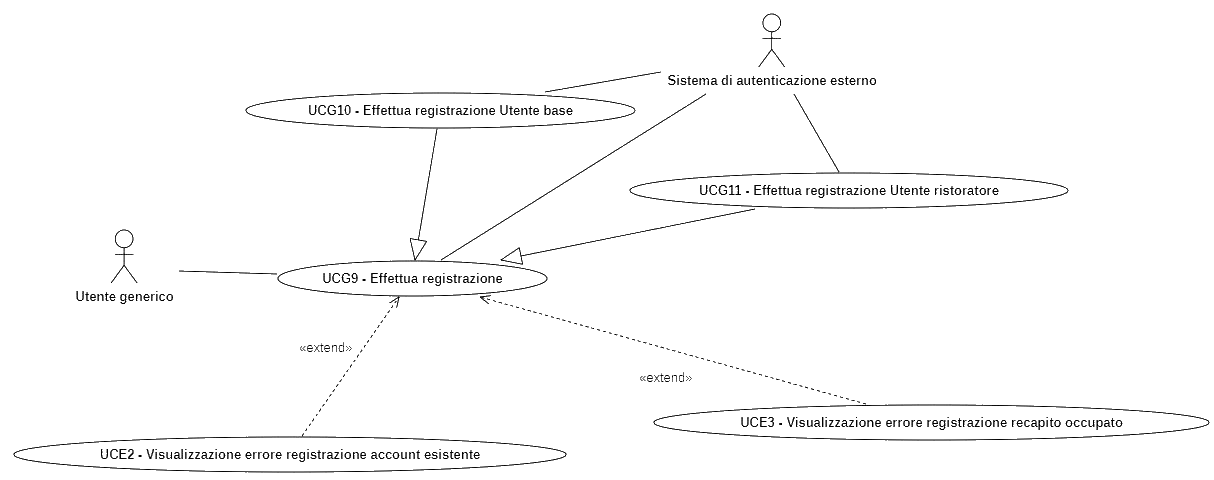
\includegraphics[width=0.99\textwidth]{./uml/UCG9-10-11.png} 
	\caption{Effettua registrazione}
	\label{fig:UCG9-10-11}
  \end{figure}

\begin{itemize}
	\item \textbf{Descrizione:} Un Utente generico decide di registrarsi all'interno della \textit{web app}. 
    Durante questa procedura, l'utente è tenuto a selezionare la tipologia di account desiderata tra le due opzioni disponibili: Utente base o Utente ristoratore. 
    Successivamente, all'utente viene richiesto di inserire una serie di dati correlati alla registrazione e specifici alla tipologia di utenza scelta.

	\item \textbf{Attore principale:} Utente generico.
	\item \textbf{Attore secondario:} Sistema di autenticazione esterno$^G$.
	\item \textbf{Precondizioni:}
        \begin{itemize}
            \item L'Utente generico è connesso al Sistema.
            \item L'Utente generico non dispone di un \textit{account}.
        \end{itemize}
	\item \textbf{Postcondizioni:}
        \begin{itemize} 
            \item L'Utente generico ha creato con successo un \textit{account} scegliendo tra le opzioni disponibili:
            \begin{itemize}
                \item Utente ristoratore.
                \item Utente base.
            \end{itemize}
            \item Tutte le informazioni relative al nuovo \textit{account} sono memorizzate all'interno del Sistema.
            \item L'utente autenticato viene reindirizzato alla pagina \textit{Home} di pertinenza.
        \end{itemize}


	\item \textbf{Scenario principale:}
	      \begin{enumerate}
		      \item L'Utente generico seleziona la tipologia di \textit{account} da creare: 
		      \begin{itemize}
				\item Utente base (vedi \autoref{usecase:Effettua registrazione Utente base}).
				\item Utente ristoratore (vedi \autoref{usecase:Effettua registrazione Utente ristoratore}).
			  \end{itemize} 
              \item Il Sistema memorizza con successo il nuovo \textit{account} creato;
		      \item L'utente è autenticato e viene reindirizzato alla pagina \textit{Home} corrispondente.
	      \end{enumerate}
		
    \item \textbf{Scenario secondario:}
                \begin{enumerate}
                    \item La registrazione fallisce per due ragioni:
                    \begin{itemize}
                        \item "La registrazione fallisce a causa dell'esistenza di un \textit{account} preesistente con le stesse credenziali inserite (vedi \autoref{usecase:Errore registrazione account esistente}).
                        \item La registrazione non va a buon fine in quanto l'Utente Ristoratore ha inserito un recapito del ristorante già occupato (vedi \autoref{usecase:Errore registrazione recapito occupato}).
                    \end{itemize}
                    \item L'Utente generico viene nuovamente indirizzato alla pagina di accesso.
                \end{enumerate}	
          
\end{itemize}
\usecaseerrore{Accesso fallito}
\label{usecase:Accesso fallito}

\begin{itemize}
	\item \textbf{Attore principale:} Utente generico.
	\item \textbf{Precondizioni:}
    L'utente ha inserito una combinazione non valida di \textit{email} e \textit{password} durante il processo di accesso.
	\item \textbf{Postcondizioni:} L'Utente generico visualizza un messaggio di errore relativo all'autenticazione fallita.

	\item \textbf{Scenario principale:}
	\begin{enumerate}
        \item Il Sistema verifica che le credenziali inserite dall'Utente base siano corrette;
        \item Il Sistema visualizza un messaggio di errore relativo all'autenticazione fallita;
        \item Il Sistema reindirizza l'Utente base alla pagina di accesso (vedi \autoref{usecase:Effettua accesso})
    \end{enumerate}
	
\end{itemize}
\usecaseerrore{Registrazione fallita}
\label{usecase:Registrazione fallita}

\begin{itemize}
	\item \textbf{Attore principale:} Utente generico.
	\item \textbf{Precondizioni:}
    L'utente durante il processo di registrazione ha:
    \begin{itemize}
        \item Inserito credenziali di un \textit{account} già esistente.
        \item Inserito le informazioni di recapito di un ristorante già esistente.
    \end{itemize}
	\item \textbf{Postcondizioni:} L'Utente generico visualizza un messaggio di errore relativo alla registrazione fallita.

	\item \textbf{Scenario principale:}
	\begin{enumerate}
        \item Il Sistema verifica che le credenziali inserite dall'Utente generico siano corrette;
        \item Il Sistema visualizza un messaggio di errore relativo alla registrazione fallita:
            \begin{itemize}
                \item Messaggio relativo all'inserito di credenziali di un \textit{account} già esistente (vedi \autoref{usecase:Errore registrazione account esistente}).
                \item Messaggio relativo all'inserimento di un recapito  di un risorante già esistente (vedi \autoref{usecase:Errore registrazione recapito occupato}).
            \end{itemize}
        \item Il Sistema reindirizza l'Utente base alla pagina di registrazione (vedi \autoref{usecase:Effettua registrazione})
    \end{enumerate}
	
\end{itemize}


\subusecase{Errore registrazione account esistente}
\label{usecase:Errore registrazione account esistente}
\begin{itemize}

	\item \textbf{Attore principale:} Utente generico.

	\item \textbf{Precondizioni:} L'Utente generico ha inserito credenziali di un \textit{account} già esistente.

	\item \textbf{Postcondizioni:} L'Utente generico visualizza un messaggio di errore relativo all'utilizzo di credenziali già in uso.

	\item \textbf{Scenario principale:}
	\begin{enumerate}
        \item Il Sistema verifica che le credenziali inserite dall'Utente generico siano corrette;
        \item Il Sistema visualizza un messaggio di errore relativo alla registrazione fallita a seguito di un utilizzo di credenziali già in uso;
	\end{enumerate}
	
\end{itemize}

\subusecase{Errore registrazione recapito occupato}
\label{usecase:Errore registrazione recapito occupato}
\begin{itemize}

	\item \textbf{Attore principale:} Utente generico.

	\item \textbf{Precondizioni:} L'Utente generico ha inserito il proprio recapito del risorante di uno già occupato.
	
	\item \textbf{Postcondizioni:} L'Utente generico visualizza un messaggio di errore relativo al recapito del proprio risorante che risulta già occupato.

	\item \textbf{Scenario principale:}
	\begin{enumerate}
        \item Il Sistema verifica che il recapito inserito dall'Utente generico sia corretto;
        \item Il Sistema visualizza un messaggio di errore relativo all'inserimento di un recapito già in uso;
	\end{enumerate}
	
\end{itemize}

%%UC DELL'UTENTE BASE

\usecasebase{Visualizzazione e modifica dati utente}
\label{usecase:Visualizzazione e modifica dati utente}
\begin{itemize}
	\item \textbf{Attore principale:} Utente base.

	\item \textbf{Precondizioni:}
	\begin{itemize}
        \item L'Utente ha eseguito correttamente l'accesso al Sistema come Utente base(vedi \autoref{usecase:Effettua accesso}).
        \item L'Utente base si trova nella propria Area Personale$^G$.
    \end{itemize}

	\item \textbf{Postcondizione:} L'Utente base visualizza e ha la possibilità di modificare i propri dati.

	\item \textbf{Scenario principale:}
	      \begin{enumerate}
		      \item L'Utente base accede alla sezione Area Personale$^G$ e sceglie di visualizzare i suoi dati personali.
		      \item Il Sistema presenta all'Utente base le seguenti informazioni:
              \begin{itemize}
                \item Nome.
                \item Cognome.
                \item \textit{E-mail}.
                \item \textit{Password}.
                \item Dettagli sulle allergie e intolleranze.
              \end{itemize}
              \item L'Utente base può  selezionare e modificare uno o più di questi dati.
              \item In caso di modifiche, il Sistema memorizza ogni variazione apportata dall'Utente base, garantendo l'integrità delle informazioni.
	      \end{enumerate}
\end{itemize}

\usecasebase{Visualizzazione storico ordini}
\label{usecase:Storico ordini}

\begin{figure}[h]
	\centering
	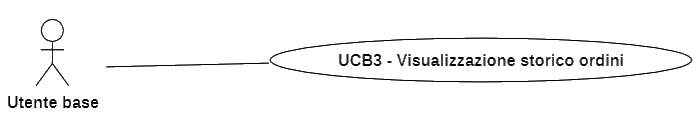
\includegraphics[width=0.8\textwidth]{./uml/UCB3.png} 
	\caption{Visualizzazione storico ordini}
	\label{fig:UCB3}
  \end{figure}

\begin{itemize}
	\item \textbf{Attore principale:} Utente base.

	\item \textbf{Precondizioni:}
	      \begin{itemize}
		      \item L'Utente ha eseguito correttamente l'accesso al Sistema come Utente base (vedi \autoref{usecase:Effettua accesso}).
		      \item L'utente deve trovarsi nella sua Area personale.
	      \end{itemize}

	\item \textbf{Postcondizione:} L'Utente base visualizza lo storico completo dei suoi ordini passati.

	\item \textbf{Scenario principale:}
	      \begin{enumerate}
		      \item Nella sezione Area personale, l'Utente base seleziona l'opzione per visualizzare lo storico dei suoi ordini;
		      \item Il Sistema presenta all'Utente base la lista degli ordini passati, ordinati cronologicamente dal più recente al meno recente.
	      \end{enumerate}
\end{itemize}


\usecase{Visualizza prenotazioni}
\label{usecase:Visualizza prenotazioni}
\begin{itemize}
	\item \textbf{Attore principale:} Utente base.

	\item \textbf{Precondizioni:}
	\begin{itemize}
        \item L'utente deve aver effettuato l'accesso (vedi \autoref{usecase:Effettua accesso}).
        \item L'utente deve trovarsi nella sua area personale.
    \end{itemize}

	\item \textbf{Postcondizioni:} L'Utente base visualizza tutte le sue prenotazioni.

	\item \textbf{Scenario principale:}
	      \begin{enumerate}
		      \item L'Utente base si trova nella sezione "area personale" e seleziona di visualizzare le proprie prenotazioni;
		      \item Il Sistema mostra tutte le prenotazioni che si trovano nel seguente stato:
              \begin{itemize}
                \item In attesa.
                \item Confermata.
                \item In corso.
              \end{itemize}
              \item L'Utente base ha una visione di tutte le prenotazioni nel corrente stato;
              \item L'Utente base può visualizzare nel dettaglio una delle prenotazioni presenti in questa lista;
	      \end{enumerate}
\end{itemize}

\usecaseautenticato{Logout}
\label{usecase:Logout}
\begin{itemize}
	\item \textbf{Attore principale:} Utente autenticato.

	\item \textbf{Precondizioni:}
	\begin{itemize}
        \item L'Utente ha eseguito correttamente l'accesso al Sistema come Utente base(vedi \autoref{usecase:Effettua accesso}).
        \item L'utente deve trovarsi nella sua Area Personale$^G$.
    \end{itemize}

	\item \textbf{Postcondizione:} L'utente esegue con successo il \textit{logout}.

	\item \textbf{Scenario principale:}
	      \begin{enumerate}
		      \item L'Utente autenticato naviga nella sezione Area Personale$^G$.
		      \item L'Utente Autenticato avvia la procedura di \textit{logout}.
              \item Il Sistema disconnette l'Utente dal suo \textit{account} e lo reindirizza alla \textit{Home} del sito, identificandolo come Utente generico.
	      \end{enumerate}
\end{itemize}

\usecasebase{Elimina account}
\label{usecase:Elimina account}
\begin{itemize}
	\item \textbf{Attore principale:} Utente base.

	\item \textbf{Precondizioni:}
	\begin{itemize}
        \item L'utente deve aver effettuato l'accesso al Sistema (vedi \autoref{usecase:Effettua accesso}).
        \item L'utente deve trovarsi nella sua area personale.
    \end{itemize}

	\item \textbf{Postcondizioni:} L'Utente base elimina il suo \textit{account}.

	\item \textbf{Scenario principale:}
	      \begin{enumerate}
		      \item L'Utente base si trova nella sezione "area personale";
		      \item L'Utente base cancella il suo \textit{account};
              \item Il Sistema cancella l'\textit{account} e tutti i dati collegato ad esso;
              \item L'utente viene riportato alla \textit{home}.
	      \end{enumerate}
	\item \textbf{Scenario secondario:}
		  \begin{itemize}
			  \item \autoref{usecase:Errore eliminazione account} Errore eliminazione account:
				\begin{enumerate}
					\item L'Utente base prova ad eliminare il suo \textit{account};
					\item Il Sistema mostra un messaggio di errore.
				\end{enumerate}
		  \end{itemize}
\end{itemize}

\usecase{Errore eliminazione account}
\label{usecase:Errore eliminazione account}
\begin{itemize}
	\item \textbf{Attore principale:} Utente base.

	\item \textbf{Precondizioni:}
	      L'Utente base si trova all'interno della selezione di eliminazione \textit{account} (vedi \autoref{usecase:Elimina account}).

	\item \textbf{Postcondizioni:}
	      L'Utente base visualizza il messaggio di errore.

	\item \textbf{Scenario principale:}
	      \begin{enumerate}
		      \item L'Utente base prova ad eliminare il suo \textit{account}.
		      \item Il Sistema visualizza il messaggio di errore che spiega che l'eliminazione non è andata a buon fine.
		      \item Il Sistema rimanda l'Utente base nella sezione di eliminazione \textit{account} (vedi \autoref{usecase:Elimina account}).
	      \end{enumerate}
\end{itemize}


\usecasebase{Prenotazione di un tavolo}
\label{usecase:Prenotazione di un tavolo}
\begin{itemize}
	\item \textbf{Attore principale:} Utente base.
	\item \textbf{Precondizioni:}
		\begin{itemize}
			\item Un Utente base ha effettuato l'accesso al Sistema (vedi \autoref{usecase:Effettua accesso});
			\item Un Utente base visualizza la pagina di dettaglio di un ristorante (\autoref{usecase:Visualizzazione di un ristorante});
		\end{itemize}
	\item \textbf{Postcondizioni:}
		\begin{itemize}
			\item L'Utente base ha confermato una prenotazione ed è tornato alla \textit{Home}.
		\end{itemize} 
	      
	\item \textbf{Scenario principale:}
	      \begin{enumerate}
		      \item L'Utente base compila una \textit{form} di prenotazione;
		      \item L'Utente base seleziona il giorno e l'ora;
		      \item L'Utente base seleziona il numero di persone;
		      \item L'Utente base inserisce eventuali necessità: particolare bisogno di seggiolini per bambini oppure se è presente un commensale con qualche disabilità o problemi di movimento;
		      \item L'Utente base inserisce lo username degli altri commensali che partecipano alla prenotazione (oppure la \textit{mail} se l'utente non è regisrato).
			  L'utente può anche decidere di non eseguire questo passaggio;
		      \item L'Utente base conferma la prenotazione.
		      \item Il Sistema registra la prenotazione.
		      \item Il Sistema crea un link condivisibile con il resto dei commensali(vedi \textit{extend:} \autoref{usecase:Condividi la prenotazione});
		      \item Il Sistema notifica la prenotazione all'Utente ristoratore (vedi \textit{extend:} \autoref{usecase:Notifica prenotazione}).
	      \end{enumerate}

	\item \textbf{Scenario secondario:}
	      \begin{itemize}
		      \item L'Utente base annulla la prenotazione (vedi
		            \autoref{usecase:Annullamento della prenotazione}).
		            \begin{enumerate}
			            \item L'Utente base annulla la prenotazione;
			            \item Il Sistema aggiorna la prenotazione.
			            \item Il Sistema notifica l'annullamento della prenotazione
			                  all'Utente ristoratore.
		            \end{enumerate}
	      \end{itemize}
\end{itemize}


\usecaseristoratore{Visualizzazione notifica prenotazione} %attore principale corretto, e colui che interagisce attivamente con la notifica. sarebbe da mettere un attore secondario DB che è colui che viene inerrogato per soddisfare il bisogno dell attore primario
\label{usecase:Visualizzazione notifica prenotazione}
\begin{itemize}
	\item \textbf{Attore principale:} Utente ristoratore.
	
	\item \textbf{Precondizione:} L'Utente base ha confermato la prenotazione ed è tornato alla \textit{Home} (vedi \autoref{usecase:Prenotazione di un tavolo}).

	\item \textbf{Postcondizione:} L'Utente ristoratore visualizza la notifica relativa ad una nuova prenotazione.
     
	\item \textbf{Scenario principale:}
	      \begin{enumerate}
                \item Il Sistema vede che al suo interno è stata fatta una nuova prenotazione;
                \item Il Sistema invia al ristoratore relativo a questa nuova prenotazione una notifica;
                \item L'Utente ristoratore visualizza la notifica relativa ad una nuova prenotazione.
	      \end{enumerate}
\end{itemize}
\usecasebase{Condividi la prenotazione}
\label{usecase:Condividi la prenotazione}
\begin{itemize}
	\item \textbf{Attore principale:} Utente base.

	\item \textbf{Precondizioni:}
	\begin{itemize}
		\item L'Utente base ha effettuato al Sistema (vedi \autoref{usecase:Effettua accesso}).
		\item L'Utente base sta visualizzando il riepilogo di una prenotazione (vedi \autoref{usecase:Visualizzazione del riepilogo prenotazione}).
	\end{itemize}

	\item \textbf{Postcondizione:}
	      L'Utente base ha copiato il \textit{link} della prenotazione e lo ha condiviso agli altri commensali.

	\item \textbf{Scenario principale:}
	      \begin{enumerate}
		      \item L'Utente base seleziona l'opzione per condividere la prenotazione;
		      \item Il Sistema mostra il \textit{link} della prenotazione;
		      \item L'Utente base copia il \textit{link} della prenotazione;
		      \item L'Utente base invia il \textit{link} agli altri utenti.
	      \end{enumerate}
\end{itemize}
\usecasebase{Annullamento della prenotazione}
\label{usecase:Annullamento della prenotazione}
\begin{itemize}
	\item \textbf{Attore principale:} Utente base.

	\item \textbf{Precondizioni:}
	      \begin{itemize}
		      \item L'Utente base ha effettuato l'accesso al Sistema (vedi \autoref{usecase:Effettua accesso}).
		      \item L'Utente base sta visualizzando il riepilogo di una prenotazione (vedi \autoref{usecase:Visualizzazione del riepilogo prenotazione}).
	      \end{itemize}

	\item \textbf{Postcondizione:}
	      L'Utente base ha annullato la prenotazione di un tavolo.

	\item \textbf{Scenario principale:}
	      \begin{enumerate}
		      \item L'Utente base seleziona l'opzione di annullamento
		            della prenotazione;

		      \item L'Utente base conferma l'annullamento della prenotazione;

		      \item Il Sistema aggiorna lo stato della prenotazione;

		      \item Il Sistema notifica l'annullamento della prenotazione
		            all'Utente ristoratore.
	      \end{enumerate}
\end{itemize}

\usecasebase{Accedi alla prenotazione}
\label{usecase:Accedi alla prenotazione}
\begin{itemize}
	\item \textbf{Attore principale:} Utente base.

	\item \textbf{Precondizione:} 
	\begin{itemize}
		\item L'Utente base è connesso al Sistema (vedi \autoref{usecase:Effettua accesso});
		\item L'Utente base ha ricevuto il link di invito ad una prenotazione (vedi \autoref{usecase:Condividi la prenotazione})
	\end{itemize}
		

	\item \textbf{Postcondizione:} L'Utente base è collegato ad una prenotazione.

	\item \textbf{Scenario principale:}
	      \begin{enumerate}
		      \item L'Utente base ha ricevuto il link di invito ad una prenotazione da parte di un altro utente;
		      \item L'Utente base accetta l'invito;
		      \item L'Utente base è ora collegato ad una prenotazione;
	      \end{enumerate}

	\item \textbf{Scenario secondario:}
		  \begin{itemize}
			  \item \autoref{usecase:Accesso prenotazione fallito} Accesso prenotazione fallito:
			  \begin{enumerate}
				  \item L'autenticazione è fallita (vedi \autoref{usecase:Accesso prenotazione fallito});
				  \item L'Utente generico viene indirizzato nuovamente nella pagina di accesso; 
			  \end{enumerate}	
		  \end{itemize}
\end{itemize}

\usecaseerrore{Accesso prenotazione fallito}
\label{usecase:Accesso prenotazione fallito}
\begin{itemize}
	\item \textbf{Attore principale:} Utente base.

	\item \textbf{Precondizione:}
	      L'Utente base accede ad una prenotazione (vedi \autoref{usecase:Accesso alla prenotazione}).

	\item \textbf{Postcondizione:}
	      L'Utente base visualizza il messaggio di errore.

	\item \textbf{Scenario principale:}
	      \begin{enumerate}
		      \item L'Utente base accetta l'invito alla prenotazione;

		      \item Il Sistema visualizza il messaggio di errore che spiega che il collegamento alla prenotazione non è andato a buon fine.
	      \end{enumerate}
\end{itemize}


\newpage
\usecasebase{Creazione dell'ordinazione collaborativa dei pasti}
\label{usecase:Creazione dell'ordinazione collaborativa dei pasti}

\begin{figure}[h]
	\centering
	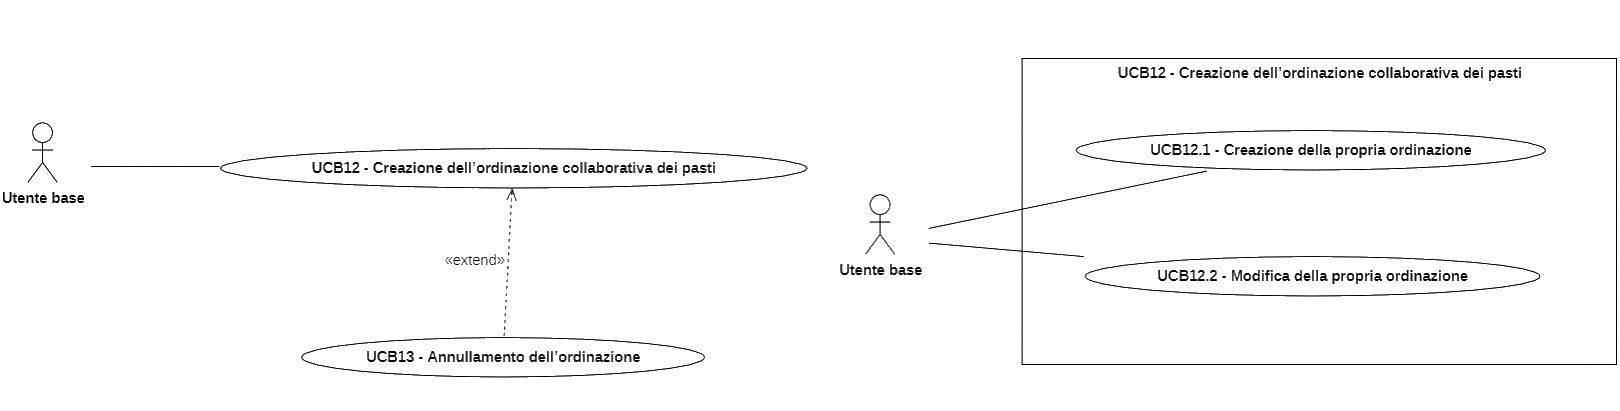
\includegraphics[width=0.9\textwidth]{./uml/UCB12-13.png} 
	\caption{Creazione dell'ordinazione collaborativa dei pasti}
	\label{fig:UCB12-13}
  \end{figure}

\begin{itemize}
	\item \textbf{Attore principale:} Utente base.

	\item \textbf{Precondizioni:}
	      \begin{itemize}
		      \item L'Utente base ha effettuato l'accesso al Sistema (vedi \autoref{usecase:Effettua accesso}).
		      \item L'Utente base ha effettuato una prenotazione (bedi \autoref{usecase:Prenotazione di un tavolo}).
		      \item L'Utente base sta visualizzando il riepilogo di una prenotazione (vedi \autoref{usecase:Visualizzazione del riepilogo prenotazione}) che si deve trovare nello stato: "Accettata"  (vedi \autoref{usecase:Accetta prenotazione}).
	      \end{itemize}

	\item \textbf{Postcondizione:} Un Utente base ha ordinato le pietanze per la prenotazione effettuata.

	\item \textbf{Scenario principale:}
	      \begin{enumerate}
		      \item L'Utente base visualizza le ordinazioni di tutti gli altri commensali collegati alla stessa prenotazione;
		      \item L'Utente base crea il proprio ordine$^G$ (vedi \autoref{usecase:Creazione della propria ordinazione});
		      \item L'Utente base modifica il proprio ordine (vedi \autoref{usecase:Modifica della propria ordinazione});

		      \item L'Utente base conferma il riepilogo dell'ordinazione;

		      \item Tutti gli Utenti base che partecipano all'ordinazione collaborativa dei pasti devono
		            confermare il riepilogo della loro ordinazione;
		      \item Il Sistema memorizza l'ordine.
	      \end{enumerate}

	\item \textbf{Scenario secondario:}
	      \begin{itemize}
		      \item L'Utente base annulla l'ordinazione (vedi
		            \autoref{usecase:Annullamento dell'ordinazione}).
		            \begin{enumerate}
			            \item L'Utente base annulla l'ordinazione;
			            \item Il Sistema aggiorna l'ordinazione.
		            \end{enumerate}
	      \end{itemize}
\end{itemize}


\subusecasebase{Creazione della propria ordinazione}
\label{usecase:Creazione della propria ordinazione}
\begin{itemize}
	\item \textbf{Attore principale:} Utente base.

	\item \textbf{Precondizione:} L'Utente base sta effettuando un ordinazione collaborativa dei pasti (vedi \autoref{usecase:Creazione dell'ordinazione collaborativa dei pasti});

	\item \textbf{Postcondizioni:}
	      \begin{itemize}
		      \item L'Utente base ha creato il proprio ordine.
		      \item Il Sistema aggiorna le informazioni inerenti al suo ordine.
	      \end{itemize}

	\item \textbf{Scenario principale:}
	      \begin{enumerate}
		      \item L'Utente base seleziona delle pietanze (vedi \autoref{usecase:Seleziona pietanza});
		      \item L'Utente base conferma il proprio ordine;
		      \item Il Sistema aggiorna il riepilogo dell'ordinazione.
	      \end{enumerate}
\end{itemize}


\subsubusecasebase{Seleziona pietanza}
\label{usecase:Seleziona pietanza}
\begin{itemize}
	\item \textbf{Attore principale:} Utente base.

	\item \textbf{Precondizione:} L'Utente base si trova nella sezione "Creazione della propria ordinazione" (vedi \autoref{usecase:Creazione della propria ordinazione}).

	\item \textbf{Postcondizione:} L'Utente base ha selezionato una pietanza.

	\item \textbf{Scenario principale:}
	      \begin{enumerate}
		      \item L'Utente base seleziona tra le lista delle pietanze una che vuole aggiungere al proprio ordine;
		      \item L'Utente base seleziona la quantità della pietanza;
		      \item L'Utente base conferma la sua selezione;
		      \item Il Sistema registra la sua selezione.
	      \end{enumerate}
\end{itemize}

\usecase{Annullamento dell'ordinazione}
\label{usecase:Annullamento dell'ordinazione}
\begin{itemize}
	\item \textbf{Attore principale:} Utente base.

	\item \textbf{Attori secondari:} Utente ristoratore.

	\item \textbf{Precondizioni:}
	      L'Utente base è connesso al sistema e si trova all'interno del caso
	      d'uso \textit{Ordinazione collaborativa dei pasti} (vedi
	      \autoref{usecase:Ordinazione collaborativa dei pasti}).

	\item \textbf{Postcondizioni:}
	      L'Utente base ha annullato l'ordinazione collaborativa dei pasti.

	\item \textbf{Scenario principale:}
	      \begin{enumerate}
		      \item L'Utente base seleziona l'opzione di annullamento
		            dell'ordinazione collaborativa dei pasti;

		      \item L'Utente base conferma l'annullamento dell'ordinazione
		            collaborativa dei pasti;

		      \item Il Sistema annulla l'ordinazione collaborativa dei pasti;

		      \item Il Sistema notifica l'Utente ristoratore e gli Utenti base
		            associati alla prenotazione collaborativa dell'annullamento
		            dell'ordinazione collaborativa dei pasti.
	      \end{enumerate}
\end{itemize}

\usecasebase{Visualizzazione del riepilogo prenotazione}
\label{usecase:Visualizzazione del riepilogo prenotazione}
\begin{itemize}
	\item \textbf{Attore principale:} Utente base.

	\item \textbf{Precondizioni:}
	\item \textbf{Precondizioni:}
	\begin{itemize}
		\item L'Utente base ha effettuato l'accesso al Sistema (vedi \autoref{usecase:Effettua accesso}).
		\item L'Utente base ha effettuato una prenotazione (bedi \autoref{usecase:Prenotazione di un tavolo}).
	\end{itemize}


	\item \textbf{Postcondizioni:}
	      L'Utente base visualizza il riepilogo della prenotazione.

	\item \textbf{Scenario principale:}
	      \begin{enumerate}
		      \item L'Utente base accede alla sezione delle prenotazioni;
		      \item L'Utente base seleziona una prenotazione;
		      \item Il Sistema mostra il riepilogo della prenotazione.
	      \end{enumerate}

	\item \textbf{Descrizione:}
	      I campi del riepilogo sono almeno:
	      \begin{itemize}
		      \item \textbf{Nome ristorante:} nome del ristorante.
		      \item \textbf{Data e ora:} data e ora della prenotazione.
		      \item \textbf{Numero di persone:} numero di persone per cui è
		            stata effettuata la prenotazione.
		      \item \textbf{Username:} username dell'Utente base
		            associato alla prenotazione o lista degli username degli
		            Utenti base associati alla prenotazione.

		      \item \textbf{Stato:} stato della prenotazione. Una
		            prenotazione si può trovare in uno dei seguenti stati:
		            \begin{itemize}
			            \item \textbf{In attesa:} la prenotazione è
			                  in attesa di conferma da parte del ristorante.

			            \item \textbf{Confermata:} la prenotazione è
			                  stata confermata dal ristorante.

			            \item \textbf{Rifiutata:} la prenotazione è
			                  stata annullata dal ristorante o dall'Utente base
			                  oppure è scaduta.

			            \item \textbf{In corso:} la prenotazione è
			                  in corso.

			            \item \textbf{Terminata:} la prenotazione è
			                  terminata e il conto è stato pagato.
		            \end{itemize}

		            Ogni volta che lo stato della prenotazione cambia, il Sistema
		            invia una notifica a tutti gli Utenti autenticati associati alla
		            prenotazione che non hanno effettuato l'azione che ha portato al
		            cambio di stato (\autoref{usecase:Notifica stato della prenotazione}).
	      \end{itemize}

\end{itemize}

\usecaseristoratore{Visualizzazione notifica nuovo ordine}
\label{usecase:Visualizzazione notifica nuovo ordine}
\begin{itemize}
	\item \textbf{Attore principale:} Sistema.

	\item \textbf{Attore secondario:} Utente ristoratore.

	\item \textbf{Precondizione:} L'Utente base ha confermato l'ordinazione collaborativa dei pasti (vedi \autoref{usecase:Ordinazione collaborativa dei pasti}).

	\item \textbf{Postcondizione:} L'Utente ristoratore visualizza la notifica relativa ad una nuova ordinazione.

	\item \textbf{Scenario principale:}
	      \begin{enumerate}
		      \item Il Sistema vede che al suo interno è stata fatta una nuova ordinazione;
		      \item Il Sistema invia all'Utente ristoratore la notifica di una nuova ordinazione;
		      \item L'Utente ristoratore visualizza la notifica relativa ad una nuova ordinazione.
	      \end{enumerate}
\end{itemize}


\usecasebase{Selezione della modalità di divisione del conto}
\label{usecase:Selezione della modalità di divisione del conto}

\begin{figure}[h]
	\centering
	
\includegraphics[width=0.9\textwidth]{./uml/UCB14.png} 
	\caption{Selezione della modalità di divisione del conto}
	\label{fig:UCB14}
  \end{figure}

\begin{itemize}
	\item \textbf{Attore principale:} Utente base.
	
	\item \textbf{Precondizione:}
	\begin{itemize}
		\item L'Utente base ha concluso l'ordinazione collaborativa dei pasti (vedi \autoref{usecase:Creazione dell'ordinazione collaborativa dei pasti}).
		\item L'Utente base visualizza il riepilogo di una prenotazione (vedi \autoref{usecase:Visualizzazione del riepilogo prenotazione}) il quale stato risulta \textit{In Corso}. 
	\end{itemize}

	\item \textbf{Postcondizione:}
	      L'Utente base ha selezionato la modalità di divisione del conto e lo ha diviso secondo le sue preferenze.
	\item \textbf{Scenario principale:}
	      \begin{enumerate}
		      \item L'Utente base seleziona la modalità di divisione del conto
		            tra quelle disponibili:
					\begin{itemize}
						\item \textbf{Divisione equa:} il conto viene diviso in parti
							  uguali tra tutti gli Utenti base che hanno condiviso la
							  prenotazione. L'Utente base può scegliere di pagare più di
							  una quota.
		  
						\item \textbf{Proporzionale:} l'Utente base seleziona i piatti che vuole
							  pagare.
					\end{itemize}

		      \item L'Utente base conferma la modalità di divisione del conto;

		      \item Il Sistema memorizza la modalità di divisione del conto.
	      \end{enumerate}

	\item \textbf{Scenario secondario:}
		  \begin{itemize}
			  \item \autoref{usecase:Visualizzazione errore divisione del conto già effettuata} Modalità di divisione del conto già effettuata:
				\begin{enumerate}
					\item L'Utente base seleziona la modalità di divisione del conto
						tra quelle disponibili;
	
					\item L'Utente base conferma la modalità di divisione del conto;
	
					\item Il Sistema mostra un messaggio di errore e spiega che la
						modalità di divisione del conto è già stata scelta.
				\end{enumerate}
		  \end{itemize}

\end{itemize}


\usecase{Modalità di divisione del conto già effettuata}
\label{usecase:Modalità di divisione del conto già effettuata}
\begin{itemize}
	\item \textbf{Attore principale:} Utente base.

	\item \textbf{Attore secondario:} Sistema.

	\item \textbf{Precondizioni:}
	      L'Utente base è connesso al sistema e ha si trova all'interno del caso
	      d'uso \textit{Selezione della modalità di divisione del conto} (vedi
	      \autoref{usecase:Selezione della modalità di divisione del conto}).

	\item \textbf{Postcondizioni:}
	      L'Utente base visualizza il messaggio di errore.

	\item \textbf{Scenario principale:}
	      \begin{enumerate}
		      \item L'Utente base seleziona la modalità di divisione.

		      \item L'Utente base conferma la modalità di divisione.

		      \item Il Sistema visualizza il messaggio di errore che spiega che
		            la modalità di divisione è già stata effettuata.
	      \end{enumerate}
\end{itemize}

\usecasebase{Pagamento del conto}
\label{usecase:Pagamento del conto}
\begin{itemize}
	\item \textbf{Attore principale:} Utente base.

	\item \textbf{Precondizione:} L'Utente base ha concluso la divisione del conto (vedi \autoref{usecase:Selezione della modalità di divisione del conto}).

	\item \textbf{Postcondizione:} L'Utente base ha pagato la sua quota.

	\item \textbf{Scenario principale:}
            \begin{enumerate}
                \item Il Sistema mostra la quota che l'Utente base deve pagare;
                \item L'Utene base seleziona la modalità con cui vuole pagare:
                \begin{itemize}
                    \item Pagare in contanti al banco.
                    \item Pagare con la carta al banco.
                    \item Pagare con buoni pasto.
                    \item Pagare in \textit{app}.
                \end{itemize}
				\item L'utente base paga la sua quota.
	      \end{enumerate}

    \item \textbf{Scenario secondario:}
		  \begin{itemize}
			  \item \autoref{usecase:Visualizzazione errore pagamento} Errore pagamento:
				\begin{enumerate}
					\item L'Utente base paga la sua quota attraverso il pagamento in \textit{app};
					\item  Il Sistema mostra un messaggio di errore.
				\end{enumerate}
		  \end{itemize}
\end{itemize}
\usecasebase{Errore pagamento}
\label{usecase:Errore pagamento}
\begin{itemize}
	\item \textbf{Attore principale:} Utente base.

	\item \textbf{Precondizioni:}
	      L'Utente base si trova all'interno della selezione del pagamento del conto (vedi \autoref{usecase:Pagamento del conto}).

	\item \textbf{Postcondizioni:}
	      L'Utente base visualizza il messaggio di errore.

	\item \textbf{Scenario principale:}
	      \begin{enumerate}
		      \item L'Utente base paga la sua quota attraverso il pagamento in \textit{app}.

		      \item Il Sistema visualizza il messaggio di errore che spiega che il pagamento non è andato a buon fine.
	      \end{enumerate}
\end{itemize}

\usecasebase{Notifica avvenuto pagamento}
\label{usecase:Notifica avvenuto pagamento}
\begin{itemize}
	\item \textbf{Attore principale:} Utente base.
	
	\item \textbf{Precondizioni:} L'Utente base ha effettuato il pagamento del suo conto (vedi \autoref{usecase:Pagamento del conto}).

    
	\item \textbf{Postcondizioni:} Il Sistema invia la notifica all'Utente ristoratore dell'avvenuto pagamento da parte del cliente.
     
	\item \textbf{Scenario principale:}
	      \begin{enumerate}
                \item Il Sistema vede che il pagamento da parte del cliente è andato a buon fine;
                \item Il Sistema invia all'Utente ristoratore una notifica dell'avvenuto pagamento;
	      \end{enumerate}
\end{itemize}

\usecasebase{Inserimento di feedback e recensioni}
\label{usecase:Inserimento di feedback e recensioni}
\begin{itemize}
	\item \textbf{Attore principale:} Utente base.

	\item \textbf{Precondizione:} L'Utente base ha completato un ordine e lo ha pagato (vedi \autoref{usecase:Pagamento del conto}).

	\item \textbf{Postcondizione:} L'Utente base ha lasciato un \textit{feedback} o una recensione.

	\item \textbf{Scenario principale:}
	      \begin{enumerate}
		      \item L'Utente base seleziona la prenotazione per la quale vuole
		            lasciare un \textit{feedback} o una recensione (vedi
		            \autoref{usecase:Visualizzazione del riepilogo prenotazione});

		      \item L'Utente base compila il \textit{form} del \textit{feedback} del ristorante;

		      \item L'Utente base conferma il \textit{feedback};

		      \item Il Sistema registra il \textit{feedback} o la recensione;

		      \item Il Sistema aggiorna la media dei punteggi del ristorante;

		      \item Il Sistema invia una notifica al ristoratore per avvisarlo
		            dell'inserimento di un nuovo \textit{feedback} o di una nuova
		            recensione (vedi \autoref{usecase:Notifica di inserimento feedback}).
	      \end{enumerate}
\end{itemize}

\usecaseristoratore{Visualizzazione notifica di inserimento \gls{Feedback}$^G$}
\label{usecase:Visualizzazione notifica di inserimento \gls{Feedback}$^G$}
\begin{itemize}
	\item \textbf{\gls{Attore}$^G$ principale:} \gls{Utente ristoratore}$^G$.

	\item \textbf{Precondizione:} L'\gls{Utente base}$^G$ ha confermato l'inserimento del \textit{\gls{Feedback}$^G$} (vedi \autoref{usecase:Inserimento di \gls{Feedback}$^G$ e recensioni}).

	\item \textbf{Postcondizione:} L'\gls{Utente ristoratore}$^G$ visualizza la notifica dell'inserimento di un \textit{\gls{Feedback}$^G$} da parte del \gls{Cliente}$^G$.

	\item \textbf{Scenario principale:}
	      \begin{enumerate}
		      \item Il Sistema vede che al suo interno è stata inserita una nuova recensione;
		      \item Il Sistema invia al ristoratore la notifica relativa all'inserimento di una recensione;
		      \item L'\gls{Utente ristoratore}$^G$ visualizza la notifica dell'inserimento di un \textit{\gls{Feedback}$^G$} da parte del \gls{Cliente}$^G$.
	      \end{enumerate}
\end{itemize}

\usecasebase{Visualizzazione della notifica di richiesta di inserimento feedback}
\label{usecase:Visualizzazione della notifica di richiesta di inserimento feedback}
\begin{itemize}
	\item \textbf{Attore principale:} Utente base.

	
	\item \textbf{Precondizione:} L'Utente ristoratore ha cambiato lo stato della prenotazione in "Terminata"(vedi \autoref{usecase:Termina prenotazione}).

    
	\item \textbf{Postcondizione:}L'Utente base visualizza la notifica in cui gli viene richiesto se vuole lasciare un textit{feedback} ad una prenotazione.
     
	\item \textbf{Scenario principale:}
	      \begin{enumerate}
                \item Il Sistema rivela un cambiamento dello stato della prenotazione;
                \item Il Sistema invia al cliente relativo a questa prenotazione una notifica in cui lo invita a lasciare un \textit{feedback};
                \item L'Utente base visualizza la notifica e dunque può:
                \begin{itemize}
                    \item Non fare nulla.
                    \item Lasciare un \textit{feedback} (vedi \autoref{usecase:Inserimento di feedback e recensioni}).
                \end{itemize}
	      \end{enumerate}
\end{itemize}

\usecase{Chat Utente base}
\label{usecase:Chat Utente base}
\begin{itemize}
	\item \textbf{Attori principali:} 
	\begin{itemize}
        \item Utente base.
        \item Utente ristoratore.
    \end{itemize}

	\item \textbf{Precondizioni:}
	\begin{itemize}
        \item L'Utente base ha acceduto al Sistema (vedi \autoref{usecase:Effettua accesso}).
        \item L'Utente base ha effettuato una prenotazione (vedi \autoref{usecase:Prenotazione di un tavolo}).
        \item L'Utente ristoratore ha effettuato l'accesso (vedi \autoref{usecase:Effettua accesso}).
    \end{itemize}

	\item \textbf{Postcondizioni:} La \textit{chat} è stata avviata.

	\item \textbf{Scenario principale:}
            \begin{enumerate}
                \item L'Utente base oppure ristoratore inizia la \textit{chat} con l'invio di un messaggio (vedi \autoref{usecase:Invio messaggio chat});
                \item Il Sistema invia una notifica l'arrivo di un nuovo messaggio al destinatario (vedi \autoref{usecase:Notifica chat}).
                \item L'utente destinatario riceve la notifica e può leggere la \textit{chat} (vedi \autoref{usecase:Lettura chat}).
                \item Ora l'Utente base e l'Utente ristoratore possono comunicare tra di loro attraverso l'uso della \textit{chat}, inviando e leggendo i messaggi vicendevolmente;
	      \end{enumerate}

    \item \textbf{Scenario secondario:}
		  \begin{itemize}
			  \item \autoref{usecase:Errore instaurazione chat} Errore instaurazione chat:
				\begin{enumerate}
					\item L'Utente base oppure ristoratore invia un messaggio in chat al destinatario.
					\item Il Sistema mostra un messaggio di errore.
				\end{enumerate}
		  \end{itemize}
\end{itemize}


%% UC UTENTE RISTORATORE
\usecaseristoratore{Consultazione lista prenotazioni}
\label{usecase:Consultazione lista prenotazioni}
\begin{itemize}
	\item \textbf{Attore principale:} Utente ristoratore.

	\item \textbf{Precondizioni:} L'Utente ristoratore ha effettuato l'accesso al Sistema (vedi \autoref{usecase:Effettua accesso}).

	\item \textbf{Postcondizioni:} L'Utente ristoratore visualizza la lista di prenotazioni (prenotazioni che si trovano in qualsiasi stato) attraverso una vista a calendario settimanale.

	\item \textbf{Scenario principale:}
	      \begin{enumerate}
		      \item Il Sistema mostra una vista a calendario settimanale, in ogni giorno della settimana l'utente può consultare:
		      \begin{itemize}
				\item La lista di prenotazioni.
				\item La lista di ingredienti con le quantità necessarie per soddisfare la richiesta giornaliera (vedi \autoref{usecase:Consultazione lista ingredienti}).
			  \end{itemize} 

		      \item Il Sistema mostra la lista prenotazioni inerente ad un giorno nei due modi seguenti:
		      \begin{itemize}
				\item Di \textit{default}, nella lista, le prenotazioni che vengono mostrate per prima sono quelle che si trovano nello stato "Accettato".
				\item L'Utente ristoratore può applicare un filtro basato sullo stato della prenotazione, per facilitare la consultazione della lista a seconda dei suoi bisogni.
			  \end{itemize}

		      \item L'Utente ristoratore visualizza la lista di prenotazioni a vista settimanale;

		      \item L'Utente ristoratore visualizza la lista degli ingredienti necessari per soddisfare a richiesta giornaliera (vedi \autoref{usecase:Consultazione lista ingredienti});
	      \end{enumerate}
\end{itemize}


\subusecase{Consultazione lista ingredienti}
\label{usecase:Consultazione lista ingredienti}
\begin{itemize}

	\item \textbf{Attore principale:} Utente ristoratore.

	\item \textbf{Precondizioni:} L'Utente ristoratore si trova nella sezione "Consultazione lista prenotazioni" (vedi \autoref{usecase:Consultazione lista prenotazioni}).

	\item \textbf{Postcondizioni:} L'Utente ristoratore visualizza la lista ingredienti aggiornata.

	\item \textbf{Scenario principale:}
	\begin{enumerate}
		\item Il Sistema mostra la lista ingredienti necessari per la giornata (relativamente alle prenotazioni nello stato "Accettata");
		\item L'Utente ristoratore visualizza la lista ingredienti;
		\item Il Sistema aggiorna costantemente la lista ingredienti (vedi \autoref{usecase:Aggiornamento lista ingredienti}) della giornata non appena l'Utente ristoratore accetta una nuova prenotazione per quella giornata;
	\end{enumerate}

\end{itemize}

\usecase{Aggiornamento lista ingredienti}
\label{usecase:Aggiornamento lista ingredienti}
\begin{itemize}
	\item \textbf{Attore principale:} Sistema.
	\item \textbf{Attore secondario:} Utente ristoratore.
	\item \textbf{Trigger:} L'Utente ristoratore ha accettato una nuova prenotazione.

	\item \textbf{Precondizioni:} 
    \begin{itemize}
        \item Il Sistema deve essere funzionante.
        \item L'Utente ristoratore ha accettato una nuova prenotazione.
    \end{itemize} 

	\item \textbf{Postcondizioni:} La lista degli ingredienti viene aggiornata.

	\item \textbf{Scenario principale:}
	      \begin{enumerate}
		      \item L'Utente ristoratore accetta una prenotazione;
		      \item Il Sistema si accorge della presenza di una nuova prenotazione accetta;
		      \item Il Sistema aggiorna la lista degli ingredienti in base alle ordinazioni presenti nella nuova prenotazione;
	      \end{enumerate}
\end{itemize}
\usecaseristoratore{Dettaglio lista prenotazioni}
\label{usecase:Dettaglio lista prenotazioni}
\begin{itemize}
	\item \textbf{Attore principale:} Utente ristoratore.

	\item \textbf{Precondizioni:} L'Utente ristoratore ha consultato la lista delle prenotazioni (vedi \autoref{usecase:Consultazione lista prenotazioni}).

	\item \textbf{Postcondizioni:} L'Utente ristoratore visualizza le prenotazioni in dettaglio.


	\item \textbf{Scenario principale:}
	      \begin{enumerate}
		      \item L'Utente ristoratore seleziona un giorno nel calendario a vista settimanale da visualizzare in dettaglio.
		      \item Il Sistema mostra tutte le prenotazioni presenti nel giorno selezionato dall'Utente ristoratore.
		      
		      \item L'Utente ristoratore seleziona una prenotazione da visualizzare in dettaglio.
		      \item Il Sistema mostra i dettagli e le informazioni relative alla prenotazione selezionata dall'Utente ristoratore:
		      \begin{itemize}
				\item Nome collegato alla prenotazione.
				\item Numero di persone.
				\item Stato della prenotazione.
				\item Giorno e l'orario della prenotazione.
				\item Eventuali persone con difficoltà motoria.
			  \end{itemize}

	      \end{enumerate}
\end{itemize}

\usecaseristoratore{Accetta prenotazione}
\label{usecase:Accetta prenotazione}
\begin{itemize}
	\item \textbf{Attore principale:} Utente ristoratore.

	\item \textbf{Precondizioni:}
	      \begin{itemize}
		      \item L'Utente ristoratore visualizza la prenotazione in dettaglio (vedi \autoref{usecase:Visualizza dettaglio lista prenotazioni}).

		      \item La prenotazione è nello stato \textit{In attesa}.
	      \end{itemize}

	\item \textbf{Postcondizione:} L'Utente ristoratore accetta la prenotazione.


	\item \textbf{Scenario principale:}
	      \begin{enumerate}
		      \item L'Utente ristoratore seleziona l'opzione di accettazione della prenotazione;

		      \item Il Sistema aggiorna lo stato della prenotazione.
	      \end{enumerate}
\end{itemize}

\usecaseristoratore{Rifiuta prenotazione}
\label{usecase:Rifiuta prenotazione}

\begin{figure}[h]
	\centering
	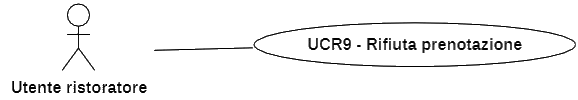
\includegraphics[width=0.9\textwidth]{./uml/UCR9.png} 
	\caption{Rifiuta prenotazione}
	\label{fig:UCR9}
  \end{figure}

\begin{itemize}
	\item \textbf{Attore principale:} Utente ristoratore.

	\item \textbf{Precondizioni:}
	      \begin{itemize}
		      \item L'Utente ristoratore visualizza la prenotazione in dettaglio (vedi \autoref{usecase:Visualizza dettaglio lista prenotazioni}).
		      \item La prenotazione è nello stato "In attesa".
	      \end{itemize}

	\item \textbf{Postcondizione:} L'Utente ristoratore rifiuta la prenotazione.



	\item \textbf{Scenario principale:}
	      \begin{enumerate}
		      \item L'Utente ristoratore seleziona l'opzione di rifiuto della prenotazione;

		      \item L'Utente ristoratore inserisce le motivazioni del rifiuto della prenotazione;

		      \item Il Sistema aggiorna lo stato della prenotazione.

	      \end{enumerate}
\end{itemize}

\usecase{Termina prenotazione}
\label{usecase:Termina prenotazione}
\begin{itemize}
	\item \textbf{Attore principale:} Utente ristoratore.

	\item \textbf{Precondizioni:} 
    \begin{itemize}
        \item L'Utente ristoratore visualizza la prenotazione in dettaglio (vedi \autoref{usecase:Dettaglio lista prenotazioni}).
        \item Tutti gli Utente base collegati alla prenotazione devono aver pagato il loro conto (vedi \autoref{usecase:Pagamento del conto}).
        \item L'Utente ristoratore riceve la notifica dell'avvenuto pagaento (ved \autoref{usecase:Notifica avvenuto pagamento}).
    \end{itemize}

	\item \textbf{Postcondizioni:} L'Utente ristoratore termina la prenotazione.


	\item \textbf{Scenario principale:}
	      \begin{enumerate}
		      \item Il Sistema mostra i dettagli della prenotazione;
		      \item L'Utente ristoratore termina la prenotazione solo nel caso in cui essa si trovi nello stato "In corso";
		      \item Il Sistema aggiorna lo stato della prenotazione.
		      \item Il Sistema aggiorna il cliente del cambio dello stato della sua prenotazione (vedi \autoref{usecase:Notifica stato della prenotazione});
		      \item La prenotazione è terminata.

	      \end{enumerate}
\end{itemize}

\usecasebase{Visualizzazione notifica stato della prenotazione}
\label{usecase:Visualizzazione notifica stato della prenotazione}

\begin{figure}[h]
	\centering
	
\includegraphics[width=0.9\textwidth]{./uml/UCB5.png} 
	\caption{Visualizzazione notifica stato della prenotazione}
	\label{fig:UCB6}
  \end{figure}

\begin{itemize}
	\item \textbf{Attore principale:} Utente base.

	\item \textbf{Precondizione:} L'Utente ristoratore ha cambiato lo stato della prenotazione (vedi \autoref{usecase:Accetta prenotazione},
	      \autoref{usecase:Rifiuta prenotazione} e \autoref{usecase:Termina prenotazione}).


	\item \textbf{Postcondizione:} L'Utente base visualizza la notifica del cambiamento di stato della sua prenotazione.

	\item \textbf{Scenario principale:}
	      \begin{enumerate}
		      \item Il Sistema rivela un cambiamento dello stato della prenotazione;
		      \item Il Sistema invia agli Utenti base relativi a questa
		            prenotazione una notifica sul cambio dello stato;
		      \item L'Utente base visualizza la notifica del cambiamento di stato della sua prenotazione, la quale si può trovare in:
		            \begin{itemize}
			            \item Accettata dall'Utente ristoratore.
			            \item Rifiutata dall'Utente ristoratore (con le motivazioni del rifiuto).
			            \item Terminata dall'Utente ristoratore.
		            \end{itemize}
	      \end{enumerate}
\end{itemize}

\usecase{Consultazione lista ordinazioni}
\label{usecase:Consultazione lista ordinazioni}
\begin{itemize}
	\item \textbf{Attore principale:} Utente ristoratore.

	\item \textbf{Precondizioni:} L'Utente ristoratore si trova a visualizzare le informazioni in dettaglio di una prenotazione (vedi \autoref{usecase:Dettaglio lista prenotazioni}).

	\item \textbf{Postcondizioni:} L'Utente ristoratore visualizza tutte le ordinazioni presenti all'interno di una determinata prenotazione.

	\item \textbf{Scenario principale:}
	      \begin{enumerate}
		      \item L'Utente ristoratore visualizza la lista delle ordinazioni di una prenotazione che si trova nello stato "Confermata" o "In corso".
		      \item Il Sistema mostra al ristoratore tutte le ordinazioni fatte dai clienti;
	      \end{enumerate}
\end{itemize}


\subusecase{Modifica ordinazione}
\label{usecase:Modifica ordinazione}
\begin{itemize}

    \item \textbf{Descrizione:} Un cliente ha un tempo limiato in cui può modificare il suo ordine, nel momento in cui lui voglia modificarlo ma ormai non sia più possibile, tale opzione di modifica è resa disponibile 
    attraverso la modifica dell'ordine da parte del ristoratore. L'utente può comunicare questa sua esigenza attraverso la \textit{chat} oppure di persona, e il ristoratore si prenderà cura di effettuare questa modifica.
	
    \item \textbf{Attore principale:} Utente ristoratore.

	\item \textbf{Precondizioni:} L'Utente ristoratore sta visualizzando la lista delle ordinazioni di una prenotazione (vedi \autoref{usecase:Consultazione lista ordinazioni}).

	\item \textbf{Postcondizioni:} L'Utente ristoratore modifica un ordinazione.

	\item \textbf{Scenario principale:}
	\begin{enumerate}
		\item L'Utente ristoratore viene a conoscenza della volontà del cliente di modificare il proprio ordine (vedi \textbf{Descrizione}).
		\item L'Utente ristoratore modifica l'ordine del cliente:
		\begin{itemize}
            \item Modifica della quantità di una pietanza all'interno dell'ordine da modificare;
			\item Rimozione di ingredienti di una pietanza all'interno dell'ordine da modificare;
			\item Aggiunta di ingredienti di una pietanza all'interno dell'ordine da modificare; 
        \end{itemize}
        \item Il Sistema notifica il cliente dell'avvenuta modifica al suo ordine attraverso una notifica (vedi \autoref{usecase:Notifica modifica ordinazione al cliente}).
	\end{enumerate}

\end{itemize}

\subusecase{Visualizza stato di pagamento}
\label{usecase:Visualizza stato di pagamento}
\begin{itemize}
	
    \item \textbf{Attore principale:} Utente ristoratore.

	\item \textbf{Precondizioni:} L'Utente ristoratore sta visualizzando la lista delle ordinazioni di una prenotazione (vedi \autoref{usecase:Consultazione lista ordinazioni}).

	\item \textbf{Postcondizioni:} L'Utente ristoratore visualizza lo stato del pagamento di un ordinazione.

	\item \textbf{Scenario principale:}
	\begin{enumerate}
		\item Il Sistema mostra per ogni ordinazione presente all'interno della prenotazione lo stato di pagamento, che può essere:
        \begin{itemize}
            \item Da pagare.
            \item Pagato.
            \item In corso.
        \end{itemize}
        \item L'Utente ristoratore visualizza per ogni ordinazione lo stato del pagamento;
	\end{enumerate}

\end{itemize}

\usecasebase{Visualizzazione notifica modifica ordinazione}
\label{usecase:Visualizzazione notifica modifica ordinazione}
\begin{itemize}
	\item \textbf{Attore principale:} Utente base.

	\item \textbf{Precondizioni:} L'Utente ristoratore ha modificato un ordinazione.(vedi \autoref{usecase:Modifica ordinazione}).

	\item \textbf{Postcondizioni:} L'Utente base visualizza la notifica relativa alla modifica della sua ordinazione.

	\item \textbf{Scenario principale:}
	      \begin{enumerate}
		      \item Il Sistema invia all'Utente base la notifica dell'avvenuta modifica al suo ordine;

		      \item L'Utente base visualizza la notifica relativa alla modifica della sua ordinazione.
	      \end{enumerate}
\end{itemize}

\usecaseristoratore{Consultazione lista feedback}
\label{usecase:Consultazione lista feedback}
\begin{itemize}
	\item \textbf{Attore principale:} Utente ristoratore.

	\item \textbf{Precondizione:} L'Utente ristoratore ha effettuato l'accesso al sistema (vedi \autoref{usecase:Effettua accesso}).

	\item \textbf{Postcondizione:} L'Utente ristoratore visualizza la lista di \textit{feedback} inseriti da vari clienti.


	\item \textbf{Scenario principale:}
	      \begin{enumerate}
		      \item Il Sistema mostra la lista di \textit{feedback};
		      \item Il Sistema mostra nome di chi ha scritto il \textit{feedback} e la data di pubblicazione;
		      \item L'Utente ristoratore visualizza tutti i \textit{feedback} e le informazioni legate ad esso.

	      \end{enumerate}
\end{itemize}

\usecaseristoratore{Segnalazione di un feedback}
\label{usecase:Segnalazione di un feedback}
\begin{itemize}
	\item \textbf{Attore principale:} Utente ristoratore.

	\item \textbf{Precondizione:} L'Utente ristoratore è entrato nella sezione di consultazione dei \textit{feedback} relativi al suo ristorante.

	\item \textbf{Postcondizione:} L'Utente ristoratore segnala al Sistema che quel \textit{feedback} non è accettabile per determinate motivazioni.


	\item \textbf{Scenario principale:}
	      \begin{enumerate}
		      \item L'Utente ristoratore segnala al Sistema un \textit{feedback} che ritiene inopportuno;
		      \item L'Utente ristoratore inserisce le motivazioni della sua segnalazione;
		      \item Il Sistema registra la segnalazione del ristoratore.

	      \end{enumerate}
\end{itemize}

\usecaseristoratore{Risposta ad un \gls{Feedback}$^G$}
\label{usecase:Risposta ad un \gls{Feedback}$^G$}
\begin{itemize}
	\item \textbf{\gls{Attore}$^G$ principale:} \gls{Utente ristoratore}$^G$.

	\item \textbf{Precondizione:} L'\gls{Utente ristoratore}$^G$ è entrato nella sezione di consultazione dei \textit{\gls{Feedback}$^G$} relativi al suo ristorante.

	\item \textbf{Postcondizione:} L'\gls{Utente ristoratore}$^G$ risponde ad un \textit{\gls{Feedback}$^G$} scritto da un \gls{Utente base}$^G$.


	\item \textbf{Scenario principale:}
	      \begin{enumerate}
		      \item L'\gls{Utente ristoratore}$^G$ risponde ad un \textit{\gls{Feedback}$^G$};
		      \item Il Sistema registra la risposta del ristoratore.

	      \end{enumerate}
\end{itemize}

\newpage
\usecasebase{Visualizzazione notifica risposta \textit{feedback}}
\label{usecase:Visualizzazione notifica risposta feedback}

\begin{figure}[h]
	\centering
	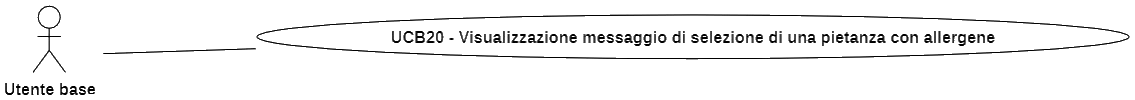
\includegraphics[width=0.9\textwidth]{./uml/UCB20.png} 
	\caption{Visualizzazione notifica risposta \textit{feedback}}
	\label{fig:UCB19}
  \end{figure}

\begin{itemize}
	\item \textbf{Attore principale:} Utente base.

	\item \textbf{Precondizione:} L'Utente ristoratore ha risposto ad un determinato \textit{feedback} (vedi \autoref{usecase:Risposta ad un feedback}).


	\item \textbf{Postcondizione:} L'Utente base visualizza la notifica relativamente ad un suo \textit{feedback}, che ha ricevuto risposta da parte del ristoratore.

	\item \textbf{Scenario principale:}
	      \begin{enumerate}
		      \item Il Sistema rivela l'inserimento di una risposta da parte del ristoratore;

		      \item Il Sistema invia una notifica all'Utente base, autore del \textit{feedback}, che ha ricevuto risposta da parte del ristoratore.
	      \end{enumerate}
\end{itemize}

\usecaseristoratore{Gestione informazioni ristorante}
\label{usecase:Gestione informazioni ristorante}
\begin{itemize}
	\item \textbf{Attore principale:} Utente ristoratore.

	\item \textbf{Precondizione:} L'Utente ristoratore ha effettuato l'accesso al Sistema (vedi \autoref{usecase:Effettua accesso}).

	\item \textbf{Postcondizione:} L'Utente ristoratore visualizza e modifica le informazioni del proprio ristorante.


	\item \textbf{Scenario principale:}
	      \begin{enumerate}

		      \item Il Sistema mostra le informazioni del ristorante:
		      \begin{itemize}
                \item Nome ristorante.
                \item Orario del ristorante.
                \item Descrizione del ristorante.
                \item Indirizzo del ristorante.
                \item Recapiti del ristorante.
                \item Password. 
                \item Link al sito del ristorante.
                \item Nome ristoratore.
                \item Costo ristorante.
                \item Disponibilità di sedie per bambini (numero).
                \item Adatto a persone con ridotta mobilità.
              \end{itemize}

		      \item L'Utente ristoratore visualizza tutte queste informazioni;
		      \item L'Utente ristoratore può modificare le seguenti informazioni;
		      \item Il Sistema registra le modifiche apporate alle informazioni dal ristoratore.

	      \end{enumerate}
\end{itemize}

\usecaseristoratore{Gestione menù}
\label{usecase:Gestione menù}
\begin{itemize}
	\item \textbf{Attore principale:} Utente ristoratore.

	\item \textbf{Precondizione:} L'Utente ristoratore ha effettuato l'accesso al Sistema (vedi \autoref{usecase:Effettua accesso}).

	\item \textbf{Postcondizione:} L'Utente ristoratore gestisce il menù del proprio ristorante.


	\item \textbf{Scenario principale:}
	      \begin{enumerate}

		      \item L'Utente ristoratore può compiere le seguenti azioni per quanto riguarda la gestione del menù:
		      \begin{itemize}
                \item Inserimento di un piatto nel menù (vedi \autoref{usecase:Inserimento piatto}).
                \item Modifica di un piatto nel menù (vedi \autoref{usecase:Modifica piatto}).
                \item Eliminazione di un piatto nel menù (vedi \autoref{usecase:Eliminazione piatto}).
              \end{itemize}
		      \item Il Sistema registra le modifiche apporate al menù da parte del ristoratore.

	      \end{enumerate}
\end{itemize}

\subusecaseristoratore{Inserimento piatto}
\label{usecase:Inserimento piatto}
\begin{itemize}

	\item \textbf{Attore principale:} Utente ristoratore.

	\item \textbf{Precondizione:} L'Utente ristoratore si trova nella sezione di gestione del menù (vedi \autoref{usecase:Gestione menù}).

	\item \textbf{Postcondizione:} L'Utente ristoratore ha inserito un piatto nel menù.

	\item \textbf{Scenario principale:}
	\begin{enumerate}
		\item L'Utente ristoratore inserisce un nuovo piatto nel menù;
		\item Il Sistema aggiorna il menù con il nuovo piatto inserito dal ristoratore.
	\end{enumerate}

\end{itemize}


\subusecaseristoratore{Modifica piatto}
\label{usecase:Modifica piatto}
\begin{itemize}

	\item \textbf{Attore principale:} Utente ristoratore.

	\item \textbf{Precondizione:} L'Utente ristoratore si trova nella sezione di gestione del menù (vedi \autoref{usecase:Gestione menù}).

	\item \textbf{Postcondizione:} L'Utente ristoratore ha modificato un piatto nel menù.

	\item \textbf{Scenario principale:}
	\begin{enumerate}
		\item L'Utente ristoratore modifica un piatto nel menù;
		\item Il Sistema aggiorna il menù con il piatto modificato dal ristoratore.
	\end{enumerate}

\end{itemize}


\subusecaseristoratore{Eliminazione piatto}
\label{usecase:Eliminazione piatto}
\begin{itemize}

	\item \textbf{Attore principale:} Utente ristoratore.

	\item \textbf{Precondizione:} L'Utente ristoratore si trova nella sezione di gestione del menù (vedi \autoref{usecase:Gestione menù}).

	\item \textbf{Postcondizione:} L'Utente ristoratore ha eliminato un piatto nel menù.

	\item \textbf{Scenario principale:}
	\begin{enumerate}
		\item L'Utente ristoratore eliminato un nuovo piatto nel menù;
		\item Il Sistema aggiorna il menù con il piatto eliminato dal ristoratore.
	\end{enumerate}

\end{itemize}

\usecaseristoratore{Modifica lista ingredienti}
\label{usecase:Modifica lista ingredienti}
\begin{itemize}
	\item \textbf{Attore principale:} Utente ristoratore.

	\item \textbf{Precondizione:} L'Utente ristoratore ha effettuato l'accesso al Sistema (vedi \autoref{usecase:Effettua accesso}).

	\item \textbf{Postcondizione:} L'Utente ristoratore gestisce la lista degli ingredienti del proprio ristorante.


	\item \textbf{Scenario principale:}
	      \begin{enumerate}

		      \item L'Utente ristoratore può compiere le seguenti azioni per quanto riguarda la gestione della lista degli ingredienti:
		      \begin{itemize}
                \item Inserimento di un nuovo ingrediente (vedi \autoref{usecase:Inserimento ingrediente}).
                \item Eliminazione di un ingrediente (vedi \autoref{usecase:Eliminazione ingrediente}).
              \end{itemize}
		      \item Il Sistema registra le modifiche apporate alla lista ingredienti da parte del ristoratore.

	      \end{enumerate}
\end{itemize}

\subusecaseristoratore{Inserimento ingrediente}
\label{usecase:Inserimento ingrediente}
\begin{itemize}

	\item \textbf{Attore principale:} Utente ristoratore.

	\item \textbf{Precondizione:} L'Utente ristoratore si trova nella sezione di gestione della lista ingredienti (vedi \autoref{usecase:Modifica lista ingredienti}).

	\item \textbf{Postcondizione:} L'Utente ristoratore ha inserito un ingrediente nella lista.

	\item \textbf{Scenario principale:}
	\begin{enumerate}
		\item L'Utente ristoratore inserisce un nuovo ingrediente nella lista;
		\item Il Sistema aggiorna la lista con il nuovo ingrediente inserito dal ristoratore.
	\end{enumerate}

\end{itemize}

\subusecaseristoratore{Eliminazione ingrediente}
\label{usecase:Eliminazione ingrediente}
\begin{itemize}

	\item \textbf{Attore principale:} Utente ristoratore.

	\item \textbf{Precondizione:} L'Utente ristoratore si trova nella sezione di gestione della lista ingredienti (vedi \autoref{usecase:Modifica lista ingredienti}).

	\item \textbf{Postcondizione:} L'Utente ristoratore ha eliato un ingrediente dalla lista.

	\item \textbf{Scenario principale:}
	\begin{enumerate}
		\item L'Utente ristoratore elimina un ingrediente dalla lista;
		\item Il Sistema aggiorna la lista con l'ingrediente che è stato eliminato dal ristoratore.
	\end{enumerate}

\end{itemize}


\usecaseristoratore{Impostazioni account ristoratore}
\label{usecase:Impostazioni account ristoratore}
\begin{itemize}
	\item \textbf{Attore principale:} Utente ristoratore.

	\item \textbf{Precondizioni:} L'Utente ristoratore ha effettuato l'accesso al Sistema (vedi \autoref{usecase:Effettua accesso}).

	\item \textbf{Postcondizioni:} L'Utente ristoratore gestisce le impostazioni del proprio \textit{account}.


	\item \textbf{Scenario principale:}
	      \begin{enumerate}

		      \item L'Utente ristoratore può compiere le seguenti azioni per quanto riguarda la gestione delle impostazioni del proprio \textit{account}:
		      \begin{itemize}
                \item Il tipo di notifiche che riceverà.
                \item Impostazioni delle \textit{chat}.
                \item Abilita modifiche ai piatti.
                \item Impostazioni \textit{feedback}.
              \end{itemize}
              \item Il Sistema memorizza qualsiasi cambiamento relativo alle impostazioni dell'\textit{account} dell ristoratore.
	      \end{enumerate}
\end{itemize}
\usecase{Chat Utente ristoratore}
\label{usecase:Chat Utente ristoratore}
\begin{itemize}
	\item \textbf{Attori principali:} 
	\begin{itemize}
        \item Utente esterno.
        \item Utente base.
        \item Utente ristoratore.
    \end{itemize}

	\item \textbf{Precondizioni:}
	\begin{itemize}
        \item L'Utente ristoratore ha effettuato l'accesso (vedi \autoref{usecase:Effettua accesso}).
    \end{itemize}

	\item \textbf{Postcondizioni:} La \textit{chat} è stata avviata.

	\item \textbf{Scenario principale:}
            \begin{enumerate}
                \item L'Utente ristoratore può iniziare la \textit{chat} con l'invio di un messaggio (vedi \autoref{usecase:Invio messaggio chat}) ad un Utente base che ha effettuato una prenotazione (ved \autoref{usecase:Prenotazione di un tavolo});
                \item Il Sistema invia una notifica l'arrivo di un nuovo messaggio al destinatario (vedi \autoref{usecase:Notifica chat}).
                \item L'Utente ristoratore riceve la notifica e può leggere la \textit{chat} (vedi \autoref{usecase:Lettura chat}).
                \item Ora l'Utente esterno/base e l'Utente ristoratore possono comunicare tra di loro attraverso l'uso della \textit{chat}, inviando e leggendo i messaggi vicendevolmente;
	      \end{enumerate}

    \item \textbf{Scenario secondario:}
		  \begin{itemize}
			  \item \autoref{usecase:Errore instaurazione chat} Errore instaurazione chat:
				\begin{enumerate}
					\item L'Utente esterno invia un messaggio in chat all'Utente ristoratore.
					\item  Il Sistema mostra un messaggio di errore.
				\end{enumerate}
		  \end{itemize}
\end{itemize}


%\section{\textit{Technology baseline}}
 % diapositiva 11 di T5
% https://www.math.unipd.it/~tullio/IS-1/2023/Dispense/T5.pdf

\section{Requisiti}
Questa sezione fornisce un elenco dei requisiti minimi indispensabili per l'esecuzione dell'applicazione, illustrando le caratteristiche necessarie per configurare 
correttamente l'ambiente di sviluppo del progetto.

\subsection{Requisiti di sistema}
Affinché l'installazione e l'avvio del prodotto avvengano senza problemi e per garantire un'esperienza completa e soddisfacente nell'utilizzo 
dell'applicazione, è essenziale installare i seguenti \textit{software}.

\begin{longtable}{|c|c|c|}
	\hline
	\textbf{Componente}       & \textbf{ Versione}   & \textbf{ Riferimenti per il download} \\
	\hline
     Node.js             & $ \geq  20.x.x$            &\href{https://nodejs.org/en/}{https://nodejs.org/en/}        \\
    \hline
     npm                & $ \geq 9.x.x$            &Integrato con il download di Node.js        \\
    \hline

    \caption{Tabella dei requisiti di sistema.}
\end{longtable}


\subsection{Requisiti \textit{software}}
L'applicazione è stata testata e confermata come utilizzabile sui principali \textit{browser}, per i quali sono specificate le versioni iniziali che hanno costituito 
il punto di partenza per lo sviluppo del progetto. Durante lo sviluppo, si è considerato incrementalmente l'aggiornamento alle versioni più recenti dei singoli \textit{browser}.

\begin{longtable}{|c|c|c|}
	\hline
	\textbf{Browser}       & \textbf{ Versione}    \\
	\hline
    Google Chrome             & 123                    \\
    \hline
    Arc                       & 1.26                    \\
    \hline
    Opera GX                       & 124                    \\
    \hline
    Safari                        & 17.3                    \\
    \hline
    Microsfot Edge                 & 123                      \\
    \hline

    \caption{Tabella dei requisiti \textit{software}.}
\end{longtable}


\subsection{Requisiti \textit{hardware}}
Poiché l'applicazione funziona su un \textit{browser}, non ci sono requisiti specifici definiti dal proponente, dal capitolato o dal progetto stesso. 
Quindi, i seguenti requisiti sono considerati solo come linee guida generali per l'esecuzione del prodotto creato.

\begin{longtable}{|l|p{0.8\textwidth}|}
	\hline
	\textbf{Componente}       & \textbf{ Requisito minimo}   \\
	\hline
     Processore             &  Processore a 64 bit Quad-Core 3,2 GHz      \\
    \hline
     Memoria RAM            &  4GB DDR4       \\
    \hline
    Spazio su disco         & $ \geq  126 GB$         \\
    \hline
    Connessione Internet         & Connessione \textit{Internet} stabile e veloce, in grado di supportare le esigenze di traffico dell'applicazione         \\
    \hline

    \caption{Tabella dei requisiti \textit{hardware}.}
\end{longtable}

\end{document}
